%%%%%%%%%%%%%%%%%%%%%%%%%%%%%%%%%%%%%%%%%%%%%%%%%%%%%%%%%%%
% EPFL report package, main thesis file
% Goal: provide formatting for theses and project reports
% Author: Mathias Payer <mathias.payer@epfl.ch>
%%%%%%%%%%%%%%%%%%%%%%%%%%%%%%%%%%%%%%%%%%%%%%%%%%%%%%%%%%%
\documentclass[a4paper,11pt,oneside]{report}
% Options: MScThesis, BScThesis, MScProject, BScProject
\usepackage[MScProject,lablogo]{EPFLreport}
\usepackage{xspace}

\title{Automatic ISA/Architecture Inference}
\author{Alex Ferragni}
%\supervisor{The PHD supervisor}
\adviser{Prof. Dr. sc. ETH Mathias Payer}
%\coadviser{Second Adviser}
%\expert{The External Reviewer}

%\newcommand{\sysname}{FooSystem\xspace}

%TODO reread: fetch address ==> fetch block
%TODO reread: be precise. "the browser..." => "the JIT compiler"

\usepackage{algorithm}
\usepackage[noend]{algpseudocode}

\begin{document}
\maketitle
%\makededication
%\makeacks

\begin{abstract}

This software security project focuses on using timing side-channels to measure cache characteristics directly from software. More precisely, it focuses on measuring both cache size and associativity on a remote machine. As opposed to previous works, the attacker model is more restrained. An attacker can only control JavaScript code, hosted in a web page. That means that the software that is executed does not need to be trusted and manually executed on a machine, since it can be executed directly in a web browser, by simply loading a web page. The software works by performing many precise memory accesses and measuring the time necessary to execute all of the accesses. Depending on the underlying cache, timing will vary, and so it becomes possible to infer information about the caches using the timing measured. In practice, this technique is more difficult when executed in a web browser, due to the more constrained environment. We will need to add a significant number of measures to be more statistically stable, and design a new iterative algorithm to progressively measure cache associativity. While it strongly depends on the underlying architecture and can easily fail on some of them, this work is sometimes capable of identifying cache sizes and precisely measuring their associativity.

%The abstract serves as an executive summary of your project.
%Your abstract should cover at least the following topics, 1-2 sentences for
%each: what area you are in, the problem you focus on, why existing work is
%insufficient, what the high-level intuition of your work is, maybe a neat
%design or implementation decision, and key results of your evaluation.
\end{abstract}

%\begin{frenchabstract}
%For a doctoral thesis, you have to provide a French translation of the
%English abstract. For other projects this is optional.
%\end{frenchabstract}

\maketoc

%%%%%%%%%%%%%%%%%%%%%%
\chapter{Introduction}
%%%%%%%%%%%%%%%%%%%%%%

%This section is usually 3-5 pages.

%The introduction is a longer writeup that gently eases the reader into your
%thesis~\cite{dinesh20oakland}. Use the first paragraph to discuss the setting.

This work will try to infer cache characteristics, namely size and associativity, directly from software. More precisely, the software will be in JavaScript and running in a web browser. For now, the browser will be either Firefox 73, or Google Chrome 79. The main method to achieve this is to measure the time necessary to execute a sequence of certain memory accesses. Depending on the underlying cache, some accesses might result in cache misses, and if we detect such misses, we can infer information about the cache.

%In the second paragraph you can introduce the main challenge that you see.

The main challenge is that JavaScript code executed from within the web browser is supposed to be isolated from the hardware it is executing on, for security reasons. That makes our objective significantly harder, since we have very limited control or knowledge about the hardware in this environment. For instance, the precision of available timers is not enough to resolve a single cache miss. Precise measures are typically necessary to infer cache characteristics. Another problem is the lack of control or knowledge about the physical translation of virtual addresses. Such lack of information makes the inference of cache associativity much more difficult, since we cannot easily choose addresses that will map to a single cache set, which is a quick way of measuring its associativity.

%The third paragraph lists why related work is insufficient.

Inferring cache size and associativity from software has already been achieved in multiple works, but all of them rely on the fact that they have access to a precise measurement system, and that they can control where virtual addresses will map to in physical memory, to some extent. The reason is that these works were implemented in more controlled environments, such as in C. None of these methods can be applied to infer cache characteristics on a machine without the need to actually control the machine in order to execute trusted code. Achieving the same capabilities in JavaScript would allow us to measure cache characteristics on a remote machine, simply by making it open a web page, which current works cannot do.

%The fourth and fifth paragraphs discuss your approach and why it is needed.

To measure cache characteristics in JavaScript, we will mostly reuse previous works, while adapting the algorithms~\cite{aleph_spectre} and methods to work with the new constraints introduced by the web browser. First off, since we do not have access to a precise clock, we need to find an alternate way to take precise measurements. Most previous works could distinguish a single cache hit from a cache miss, but it turns out this much precision is not necessary. It is possible to modify previous algorithms to use another measurement system that can only tell, among many memory accesses, whether some misses occurred, or only hits occurred. This new relaxed measurement system is in fact implementable in JavaScript, by chaining misses to amplify their impact on timing, and carefully choosing a set of addresses to work with.

%contd.

A second problem comes from the fact that we do not know where virtual memory in a browser is mapped to in physical memory. Previous works relied on the fact that they could take precise measures, or they could choose a set of addresses that were all mapped to the same cache set, i.e., by using huge pages, or simply by only measuring small enough caches. Unfortunately, we cannot directly achieve this in a browser, due to the limited control. This does not pose a problem while measuring cache size, but it becomes more complicated to measure cache associativity. While the associativity of the first level cache can still be measured by reproducing some previous work~\cite{eviction_sets} and isolating an eviction set, this method cannot be applied to the following caches. We will need to design a new algorithm that will iteratively find eviction sets. By using an iterative approach, we can progressively gain knowledge about the addresses we are using, and eventually recover enough information to find an eviction set for every single data cache, including the last shared cache.

%The sixth paragraph will introduce your thesis statement. Think how you can
%distill the essence of your thesis into a single sentence.

In summary, measuring cache size and associativity is already possible in software, as previous works showed~\cite{abel}. Unfortunately, they require control over the victim machine. 
This work thus tries to modify some previously done cache inference algorithms to make them work in a less controlled and more realistic environment, namely executed in a web browser. 
We will need to find solutions to new problems introduced by the lack of control we have from within the web browser.

%The seventh paragraph will highlight some of your results

By amplifying cache misses, we can implement some existing algorithms in JavaScript and get a direct measure of both cache size and associativity on some machines. For instance, when executed on an Intel Core i7-4870HQ processor using Google Chrome, the algorithm could successfully detect three caches, of size close to 32KB, 256KB and 6MB respectively. Furthermore, the new iterative algorithm could determine that their associativity is 8, 8 and 12 respectively, despite the fact that the last cache is sliced and shared across cores. When executed on an Intel Core i7-8700, it could successfully measure that the associativity of the last level cache is 16.

%The eights paragraph discusses your core contribution.

Finally, we summarize here the contributions of this work. We took an existing algorithm~\cite{abel} to measure cache size in software, and adapted it to work in JavaScript, using part of an existing way to take precise measures in JavaScript~\cite{aleph_spectre}, allowing it to be executed more easily, on a remote machine. Similarly, we took an algorithm to measure a cache associativity, and adapted it to measure the first level cache associativity in JavaScript. Furthermore, we designed an algorithm capable of measuring the associativity or the following caches in JavaScript, without the need to control or monitor the physical translation of virtual addresses, or to have precise measures, unlike previous works.

%%%%%%%%%%%%%%%%%%%%
\chapter{Background}
%%%%%%%%%%%%%%%%%%%%

%The background section introduces the necessary background to understand your
%work. This is not necessarily related work but technologies and dependencies
%that must be resolved to understand your design and implementation.

%This section is usually 3-5 pages.

\section{Caches}

%TODO: (here also)

Caches were introduced in processors to speed up memory accesses. The reason is that caches serve as a memory/speed trade off. Caches are smaller than the main memory, but are also faster to access. They are mostly organized in hierarchy. When the processor wants to fetch a block from memory, it first checks whether it is contained in the \emph{first level cache} (L1). The L1 is the fastest but smallest cache. If the block is not contained in the L1, it will then check the other caches, or finally the main memory if no cache contains it. Each cache has a greater capacity, but also slower accesses than the previous one. Finally, the \emph{last level cache} (LLC) is often shared across cores, and cache coherence protocols maintain a coherent state of the cache across cores.

\begin{figure}
    \centering
    \fbox{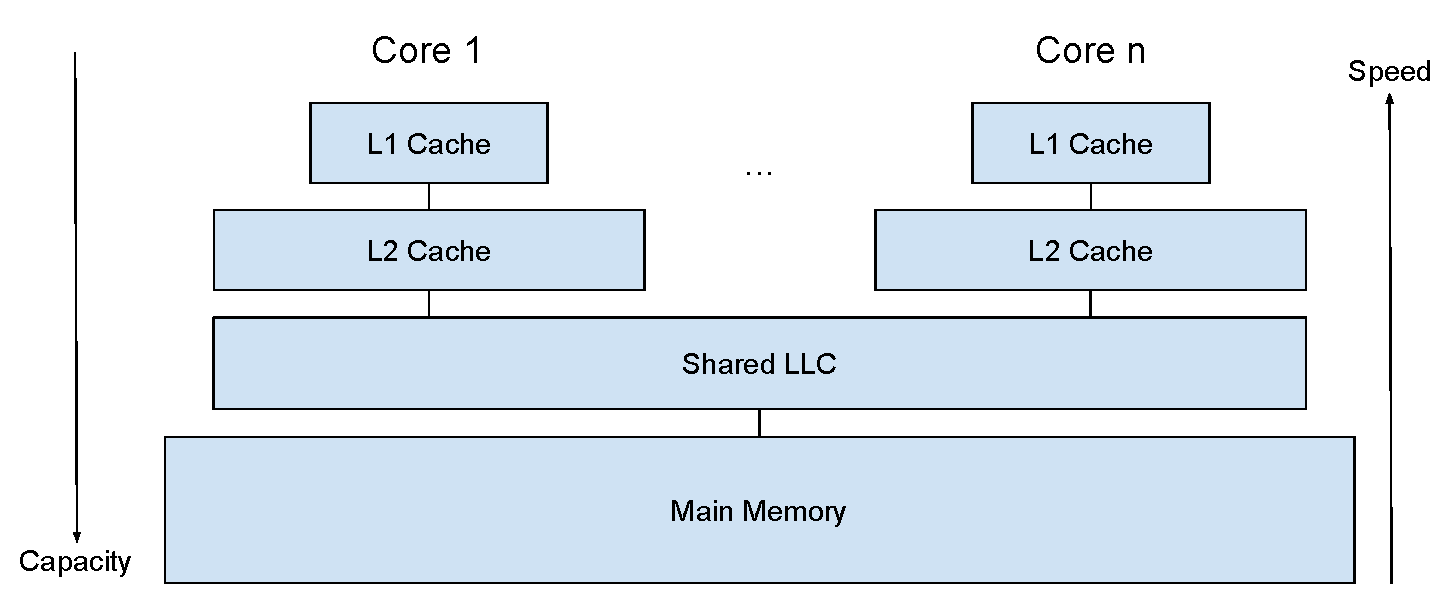
\includegraphics[width=15cm]{figures/illustrations/cache_hierarchy.pdf}}
    \caption{Conceptual view of the cache hierarchy on a computer with n cores and three cache levels}
    \label{fig:cache_hierarchy}
\end{figure}

We call \emph{cache hit} or simply \emph{hit} when the processor fetches a block that is contained in the cache. Similarly, we call \emph{cache miss} or \emph{miss} when the block is not contained in the cache, and it has to be fetched from a slower cache, or from memory. A cache hit is thus faster than a cache miss.

A cache typically has some level of associativity, which represents the number of conflicting block it can still contain. If a cache is $n$-associative, then it is separated into $n$ parts we call \emph{ways}. The L1 cache is virtually indexed, meaning that when a block needs to be fetched, the lower order bits of its virtual address will indicate where in a way it will map to. The other caches (L2, LLC) are physically indexed, meaning that the physical translation of this virtual address indicates the cache set the block will map to. The cache will then check in every way if the block is contained, and can otherwise choose in which way the block will be stored. To distinguish blocks in the caches, they keep track of tags, which are composed of higher order bits of the physical addresses, meaning the caches are physically tagged.

\begin{figure}
    \centering
    \fbox{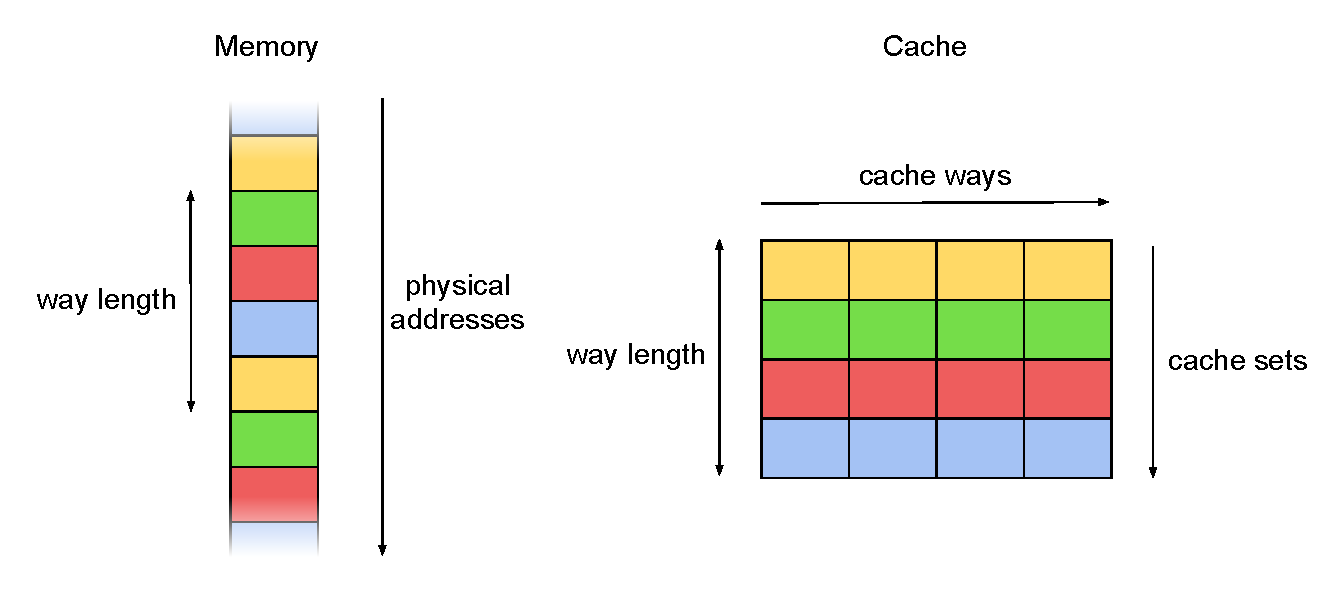
\includegraphics[width=15cm]{figures/illustrations/cache_associativity.pdf}}
    \caption{Conceptual view of the associativity of a cache}
    \label{fig:cache_associativity}
\end{figure}

"Evaluating associativity in CPU caches"~\cite{3C} distinguishes three types of misses. A compulsory miss happens when a block is first loaded, it cannot initially be in a cache, and it results in a compulsory miss. A capacity miss happens when we are accessing more blocks than the cache can physically hold. If the cache is full and needs to load another block, then there is a capacity miss. A conflict miss happens when we are accessing more conflicting blocks than the cache can hold, even though the cache might not be full. If we try to access a number of blocks which all map to the same cache set that is greater than its associativity, then there will be conflict misses.

When a conflict miss or capacity miss happens, the cache has to clear one of its cache line, to make room for the data that caused a miss. The cache eviction policy is the algorithm that will decide which line to evict when necessary, depending on the current cache state.

Finally, we call \emph{eviction set} a set of virtual addresses that will always result in conflict misses, if we access the entire set consecutively.

\section{TLB}

When a virtual address needs to be loaded from memory or from a cache, it first needs to be translated to a physical address. This translation may require several memory accesses. This is where the \emph{Translation Lookaside Buffer} (TLB) comes in play. Its purpose is to store some recent translations, to avoid translating them again and speed up the process by avoiding some memory accesses. The TLB acts like a cache, meaning it has a certain capacity and associativity, but as opposed to a real cache, it stores virtual address translations. 

This means that if an address is not contained in the TLB, a TLB miss will occur, whereas if it were in the TLB, a TLB hit would have occurred. Again, a TLB miss is slower than a TLB hit. Then finally, after the translation, the physical address will be looked up in the caches or the memory.

\section{Huge Pages}

Most modern processors, including our targets, use paging-based virtualization. Each virtual \emph{page} is then individually mapped to a physical page, meaning that physical translations of contiguous virtual addresses might not be contiguous anymore. Within a single page though, addresses are still consecutive in physical memory.

Some architectures supports so-called huge pages, which can be MB or even GB big. Using huge pages greatly reduces time necessary to translate addresses and is useful for some specific programs, but it also means that those programs can have more information about physical translation of the virtual addresses they use. With 4KB pages, a program can only control addresses within a 4KB page, but with 1GB huge pages, it becomes possible to allocate a 1GB virtual region that will be entirely consecutive in physical memory as well, which would give more control to a program. 

That much control over physical addresses can be harmful for a machine, if the program being executed is malevolent, thus in practice huge pages must be explicitly enabled and allowed for a program to use them. This means that it is not possible to use huge pages directly in a JavaScript code executed in a browser in general, since some machines might simply disable them for security reasons.

\section{Browser Limitations}

When a web page containing some JavaScript code is loaded on a web browser, the code it contains should be executed on the machine. Unfortunately, this code cannot be executed directly, as it could be dangerous. In fact, it is fairly easy to host a web page containing some code, and so we cannot expect to trust every web page. Some could contain faulty code, or even malicious code. Therefore, a computer cannot simply execute all JavaScript code contained in the web pages directly for security reasons.

The code cannot directly be executed on the machine, but there is still a safer way to execute it. Web browsers introduce a way to execute JavaScript code in a sandbox. The reason is that in an isolated environment, the code loses both impact and control over the machine it is being executed on. This way, the code can only access the machine via the web browser, which means that the browser can control what the code can or cannot do. The JavaScript code does not have access to sensitive information that could be dangerous and lead to an attack on that machine. Such information include most hardware characteristics, the computer's file system, or even a precise processor clock. 

The code also suffers from the fact that the browsers controls the execution. More precisely, the \emph{just-in-time} (JIT) compiler can decide to modify the code for performance or security reasons. For this reason, it is difficult to control the execution of the code, even if it is possible to manipulate the behaviour of the JIT compiler from within the code, in some cases. 

Even some functionalities that do not directly leak information can be controlled by the browser. As instance, the code can access a clock, but it is provided by the browser, so the latter is free to reduce its precision and add jitter to limit the capabilities of the code. The JIT compiler also have full control over physical memory, while the code has close to none. From the code, it is not directly possible to choose where a virtual address will be mapped to in physical memory, neither is it to track the virtual to physical translation.

%%%%%%%%%%%%%%%%
\chapter{Design}
%%%%%%%%%%%%%%%%

%Introduce and discuss the design decisions that you made during this project.
%Highlight why individual decisions are important and/or necessary. Discuss
%how the design fits together.

%This section is usually 5-10 pages.

\section{Precise Measurement System}

Since no provided clock is precise enough to distinguish a cache miss from a cache hit, we need to amplify cache misses. To do so, we will find a sequence of accesses that will have different hit rates depending on an hypothesis. We will build it so that the hit rate is equal to 100\% if and only if a certain block results in a cache hit. This way, if we have enough consecutive memory accesses, we can measure their cumulative time, and the time difference between the two executions can then be made greater than the resolution of the provided clock, and so we can distinguish the two cases. \autoref{fig:measurement_system} summarizes this.

The technique we will use in the experiments is to keep track of a set of virtual addresses (which we will call \emph{measure set}), and to measure the time it takes to do a fixed number of memory accesses from this set. By progressively adding addresses to this set and repeat the measures, we can then tell whether the new address caused misses or not by detecting a sudden increase in the time measured. By having more assumptions on the addresses we are accessing, we will identify the misses that occur more precisely.

\begin{figure}
    \centering
    \fbox{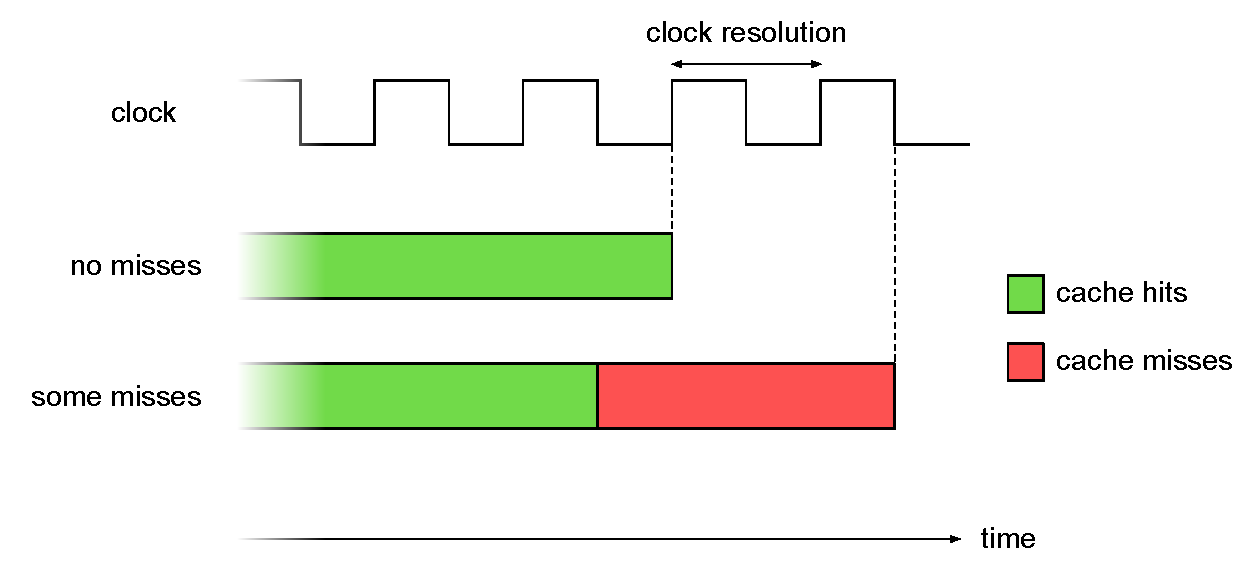
\includegraphics[width=15cm]{figures/illustrations/measurement_system.pdf}}
    \caption{Detecting cache misses}
    \label{fig:measurement_system}
\end{figure}

Further increasing the number of accesses and taking the average over multiple experiments is a good way to get more consistent measures. It is necessary to do so, given the amount of noise that is interfering with the measures.

\subsection{Prevent Optimizations}

Modern web browsers and processors have to make sure they are efficient and secure, thus different optimizations are often implemented. These optimizations may tamper with our measurement system, so we need to prevent them. Most of these techniques have been described in previous work~\cite{aleph_spectre}.

\subsubsection{Instruction Pipelining}

Modern processors are \emph{out-of-order} (OoO). The main advantage is that is can greatly increase throughput of a processor. A consequence is that while a memory instruction waits for its result, other independent instructions can be executed as well. This means, for example, that if we try to execute multiple independent reads, then they may be executed in parallel, and the throughput will be greatly increased. This is undesirable as we need to precisely measure the time needed to perform the memory accesses, we want memory instructions to be executed one after the other.

To fix that issue, we introduce dependencies between the reads. If the result of a read is necessary to determine the address of the next read, then the processor will not parallelize the memory accesses, and they will be executed in a serialized way.

\subsubsection{Hardware Prefetching}

Another problem is that when a sequence of addresses is being accessed, if the sequence is predictable enough, the processor might dynamically recognise the access pattern, and subsequently prefetch the next blocks in the sequence. This way, it might avoid further misses if the access sequence was correctly recognized.

To avoid this optimisation, we need to make sure that successive memory loads are not accessing addresses consecutively. In fact, we will make sure that the order of the accesses looks "random", to ensure that no optimisation can "guess" and load in advance the next block.

\subsubsection{Dead Code Elimination}

Dead code elimination happens when a piece of code carries no useful result, and removing this piece of code would have no effect on the rest of the program. The JIT compiler could then simply ignore this code and avoid wasting time and resources. The problem is that our main measurement method measures the time we need to do many memory accesses, but they do not carry any result, and so they could be optimized away, which would make our program useless. 

To solve this, we will need to carry the results of the loads and modify the output of the program depending on their results. This way, the JIT compiler cannot optimize the memory accesses away without modifying the program result.

\section{Measure Cache Size}
\label{sec:measure_cache_size}
A first simple objective is to measure the size of different caches. It is done using the fact that a cache cannot contain more than its capacity, and whenever we access more than its capacity, there have to be cache misses. 

From this fact, we use a straight-forward method to detect the cache size. The idea is to measure the time taken to perform a constant number of memory accesses on a region of fixed size. We can then progressively increase the size of this region, and repeat the measures. \autoref{fig:cache_size} depicts the moment where cache misses start occurring. In Case 1, the measure set is still entirely contained by the cache, there are only cache hits. In Case 2, we added another address to the measure set, thus making the measure set overflowing from the cache, which means cache misses will start to occur.

\begin{figure}
    \centering
    \fbox{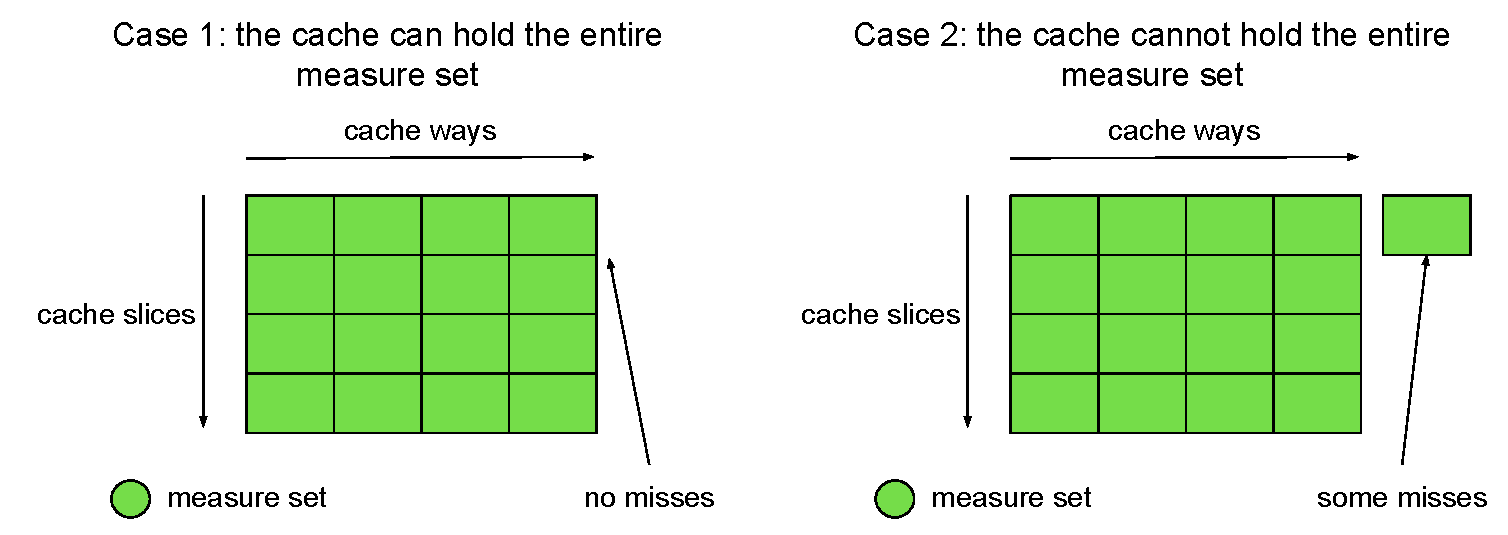
\includegraphics[width=15cm]{figures/illustrations/cache_size.pdf}}
    \caption{Measuring the cache size}
    \label{fig:cache_size}
\end{figure}

With this method, we expect to see an increase in the slope of the times measured whenever we are using a region which size is close to a cache capacity. Indeed, we expect the behaviour of the function to be the following one: while the region is smaller than any cache, the whole region can fit in the L1 cache, and no misses occur, the time should be constant. When the region size gets close to the L1 capacity, we expect to see L1 misses, and the time should increase. As the region grows, the hit ratio will decrease, and eventually stabilize around 0\%, when the time function should again be relatively constant. The same phenomenon happens around the capacity of the L2 cache: we transition from a state where we have L1 misses and L2 hits to a state where we have both L1 and L2 misses. The same applies to every subsequent cache, although we expect much more noise with the LLC, since it is shared and potentially suffers from cache pollution.

In practice, the results might differ a bit from theory in an environment without control over physical addresses of the virtual region. If it were contiguous in memory, then addresses would be evenly distributed among cache sets, and we would effectively completely fill up a cache before having cache misses. In our case, contiguous virtual addresses may not be distributed evenly among cache sets. In consequence, it is possible to observe cache misses before reaching the capacity of the cache, and the measures will thus be a bit imprecise. In practice, the difference between the cache size and the measure differs by at most a factor of two.

\section{Measure Cache Associativity}
\label{sec:measure_associativity}

Another objective is to measure the associativity of the different caches of a computer. This work has been done already~\cite{tlb_characteristics}, but the web browsers introduce some new limitations that we have to deal with .
The main limitations are the lack of control over physical addresses and precise measurement methods, due to the fact that the script is executed by a web browser.

\subsection{With physical contiguous memory}
\label{sec:llc_eviction_simple}
In a simpler model where virtual memory is mapped to a contiguous area in physical memory, an algorithm to detect cache associativity is fairly simple and has been done already, even when it comes to measuring the associativity of the LLC.

The key idea is that we can control which virtual addresses will map to a certain cache set, since virtual addresses stay contiguous. Indeed, we know that to determine which cache set an address will map to, only a certain number of lower order bits of the address are taken into account. In other words, if an address is shifted by a multiple of a big enough value, then the corresponding cache set remains the same. The minimum such shift is the size of a way of the cache, i.e., the capacity of the cache divided by its associativity.

We also know that if we are accessing a number of blocks that is bigger than the associativity of the cache, and if they all map to the same cache set, then the cache cannot hold them all, and there will necessarily be cache misses. This gives us a way to simply measure its associativity, and it requires very few addresses to work. \autoref{fig:associativity_simple} depicts the moment where adding an additional address in the measure set will result in cache misses.

\begin{figure}
    \centering
    \fbox{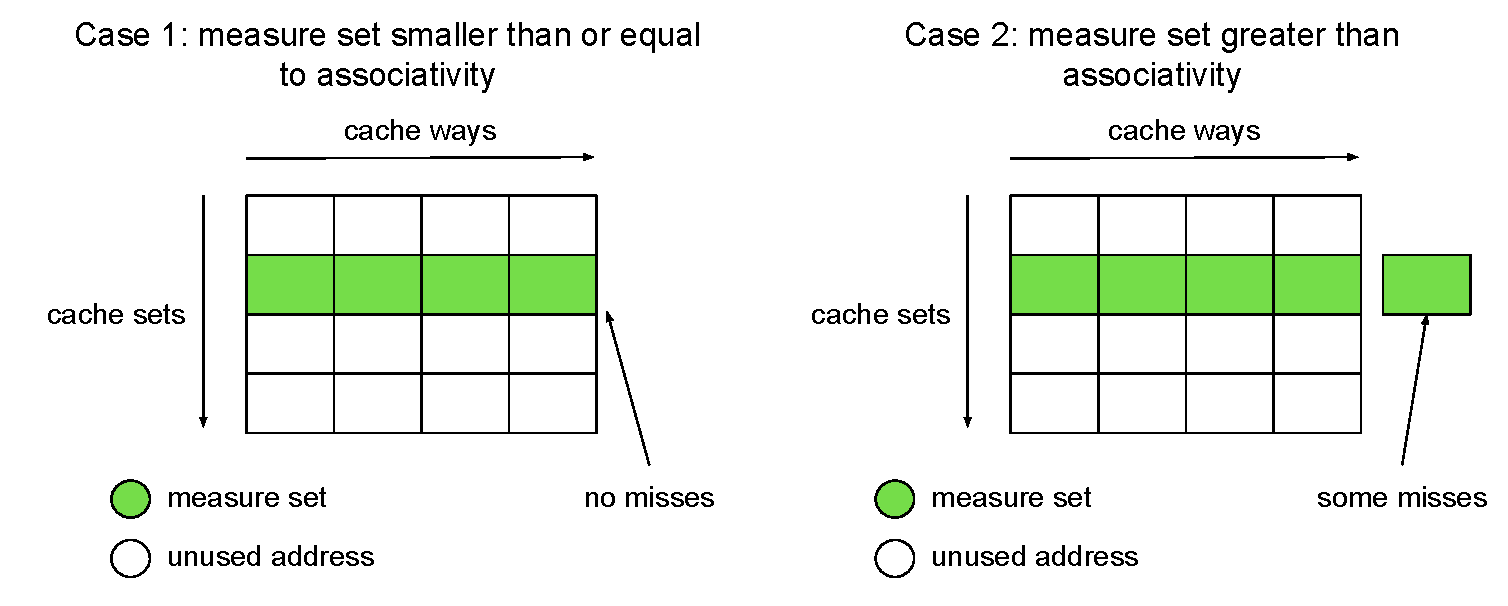
\includegraphics[width=15cm]{figures/illustrations/associativity_simple.pdf}}
    \caption{Finding the associativity of a cache, with contiguous memory}
    \label{fig:associativity_simple}
\end{figure}

When it comes to measuring the associativity of the LLC, things get more complicated. The main problem is that the LLC is often split in multiple slices, and each slice acts as a separate cache. Even if we can control in which cache set a block will mapped to, we do not know in which slice it will be mapped. It would then be possible to access a number of blocks that is bigger than the associativity of the cache, while all of them map to the same cache set, and still observe no cache misses, since they could map to different slices.

Nonetheless, there is a maximum number of blocks this cache can hold. After a certain number of accesses, one of the slices will be full, no matter how addresses are mapped to slices, and we will then observe cache misses. We will need to recover which blocks map to the slice that overflowed, to then find its associativity. Therefore, the same method can be applied for the LLC: using an increasing number of addresses, and detecting a step in the time function. \autoref{fig:associativity_simple_llc} depicts the moment where adding another address in the measure set results in a slice overflowing, causing cache misses.

\begin{figure}
    \centering
    \fbox{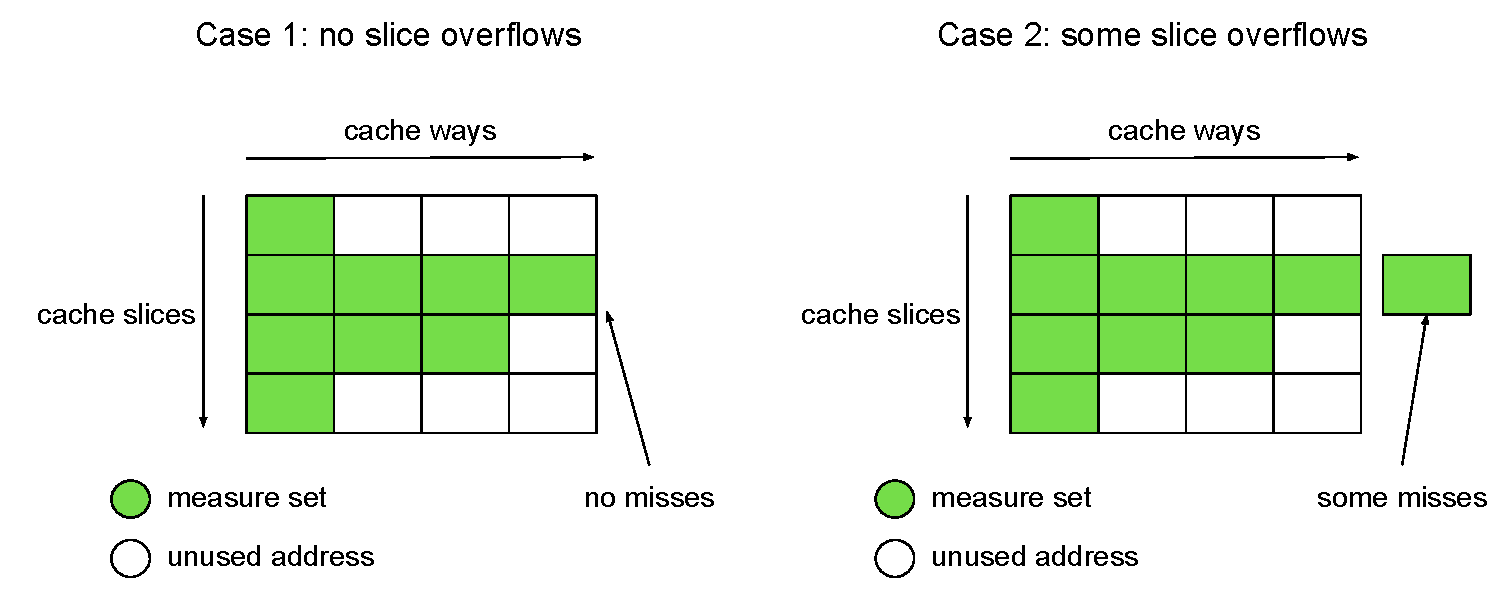
\includegraphics[width=15cm]{figures/illustrations/associativity_simple_llc.pdf}}
    \caption{Finding an LLC eviction set, with contiguous memory}
    \label{fig:associativity_simple_llc}
\end{figure}

Once the step is detected, we know that exactly one slice overflows, since we detected the first LLC misses. From there, it is possible to recover the exact eviction set by observing the behaviour of a measure when removing a single address from the set. If we take measures with the entire current set, we know there are cache misses. But if we remove a single address from this set and take measures again, this might not be the case anymore. If the block we removed was not in the slice that overflowed (i.e., it was not in the eviction set), then the slice is still overflowed. This means that if we then take measures, there will be LLC misses. On the other hand, if the address we removed was in the overflowing slice, then we just removed an block from this slice, which means that it does not overflow anymore. Furthermore, we know the other slices do not overflow, thus it we then take a measure, there will be no LLC misses. \autoref{fig:isolate_eviction} summarizes this procedure. In Case 1, the candidate address belongs to the eviction set, but since the candidate address is ignored during the measure, the slice does not overflow anymore, and there are no cache misses. In Case 2, the candidate address does not belong to the eviction set, and so removing it does not prevent cache misses from occurring.

\begin{figure}
    \centering
    \fbox{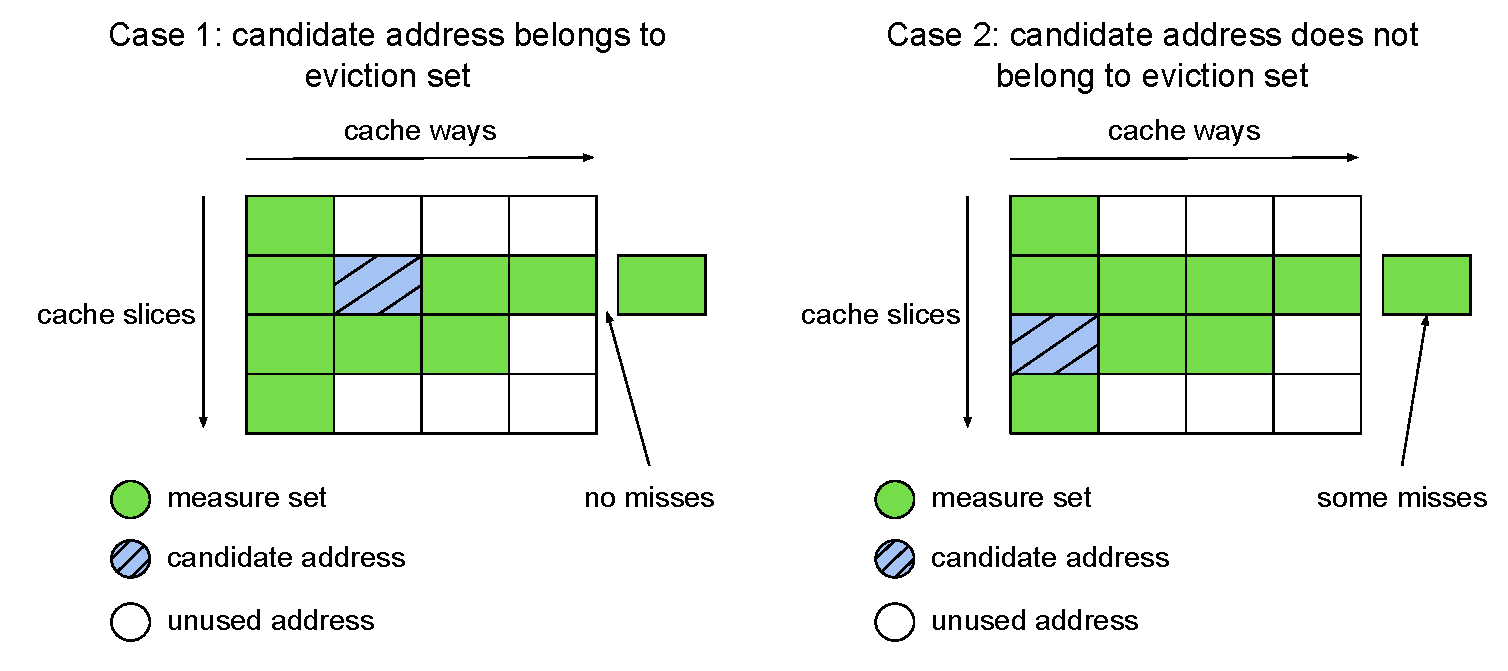
\includegraphics[width=15cm]{figures/illustrations/isolate_eviction.pdf}}
    \caption{Isolating the eviction set}
    \label{fig:isolate_eviction}
\end{figure}

To summarize, if we remove a single address from the measure set, the presence of LLC misses or not should indicate whether this address is in the eviction set. To isolate the eviction set, it follows that we should repeat the procedure for every address in our set: remove the current address from the set, take a measure, and put it back in. The time measured should then be separated into two clusters, corresponding to the presence or not of LLC misses. The cluster of faster measures then corresponds to the eviction set, and its size indicates the associativity of the LLC.

\subsection{Without physical contiguous memory}
\label{sec:cache_associativity_no_contig}

The previous method only works if the block map to the same cache set, as we assumed earlier. In practice, we have no control over the physical location of virtual memory in a web browser. In fact, we are not even guaranteed that two virtual addresses separated by a multiple of the page size will also be separated by a multiple of the page size in physical memory.

Thus, we need to design another algorithm to get a measure of the associativity of the caches. The previous method was designed to isolate addresses that map to a single slice, among a group of other different slices. In the same way, it can be used to differentiate addresses that map to a certain cache set, among addresses that map to different cache sets. Indeed, if the previous method is applied without assumption on the physical addresses, we will still eventually observe some cache misses, and we will detect an eviction set, but it will most probably correspond to a L1 eviction set. 

With this eviction set, we get a measure of the associativity of the L1, but we also get a way to tell whether an arbitrary virtual address maps to the same cache line as our eviction set or not. By measuring the time taken to access the entire eviction set as well as our candidate address, we can tell whether it maps to the same cache line. If the candidate belongs to this set, then there will be cache misses. If it does not, there will only be hits. It follows that the time measured can indicate whether an address belongs to this eviction set.

\begin{figure}
    \centering
    \fbox{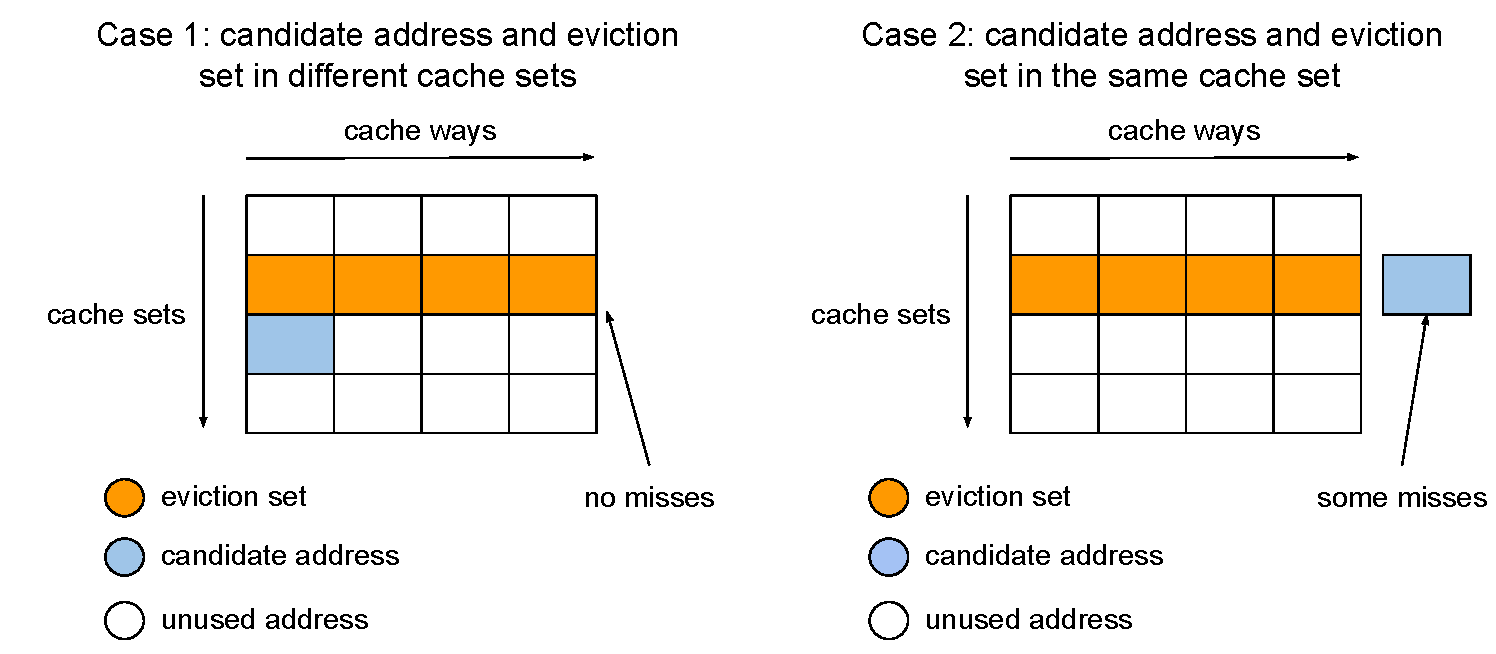
\includegraphics[width=15cm]{figures/illustrations/eviction_oracle.pdf}}
    \caption{Using the eviction set as an oracle}
    \label{fig:eviction_oracle}
\end{figure}

\autoref{fig:eviction_oracle} summarizes the procedure to check whether a candidate address belongs to the same cache set as the eviction set. It is done by taking a measure, using as measure set the eviction set as well as the candidate address. If the candidate address belongs to a different cache set (Case 1), the entire measure set fits in the cache, and we expect no misses. But if the candidate address belongs to the same cache set (Case 2), the measure set cannot fit entirely in the cache, and there will be cache misses during the measure, which we will detect.

Using this oracle, we can filter out all the addresses that do not map to the same L1 set, and only keep the remaining addresses. This means that we can now find a set of addresses we know will map to the same L1 set. With that, we greatly reduce the noise caused by the L1 cache while trying to measure the associativity of the next caches. Indeed, if we try to access addresses that all map to the same L1 set, there is a single number of addresses from which we will start to observe L1 misses, and we know precisely when this will happen, so we can ignore it. It will be easier to observe L2 misses this way.

\begin{figure}
    \centering
    \fbox{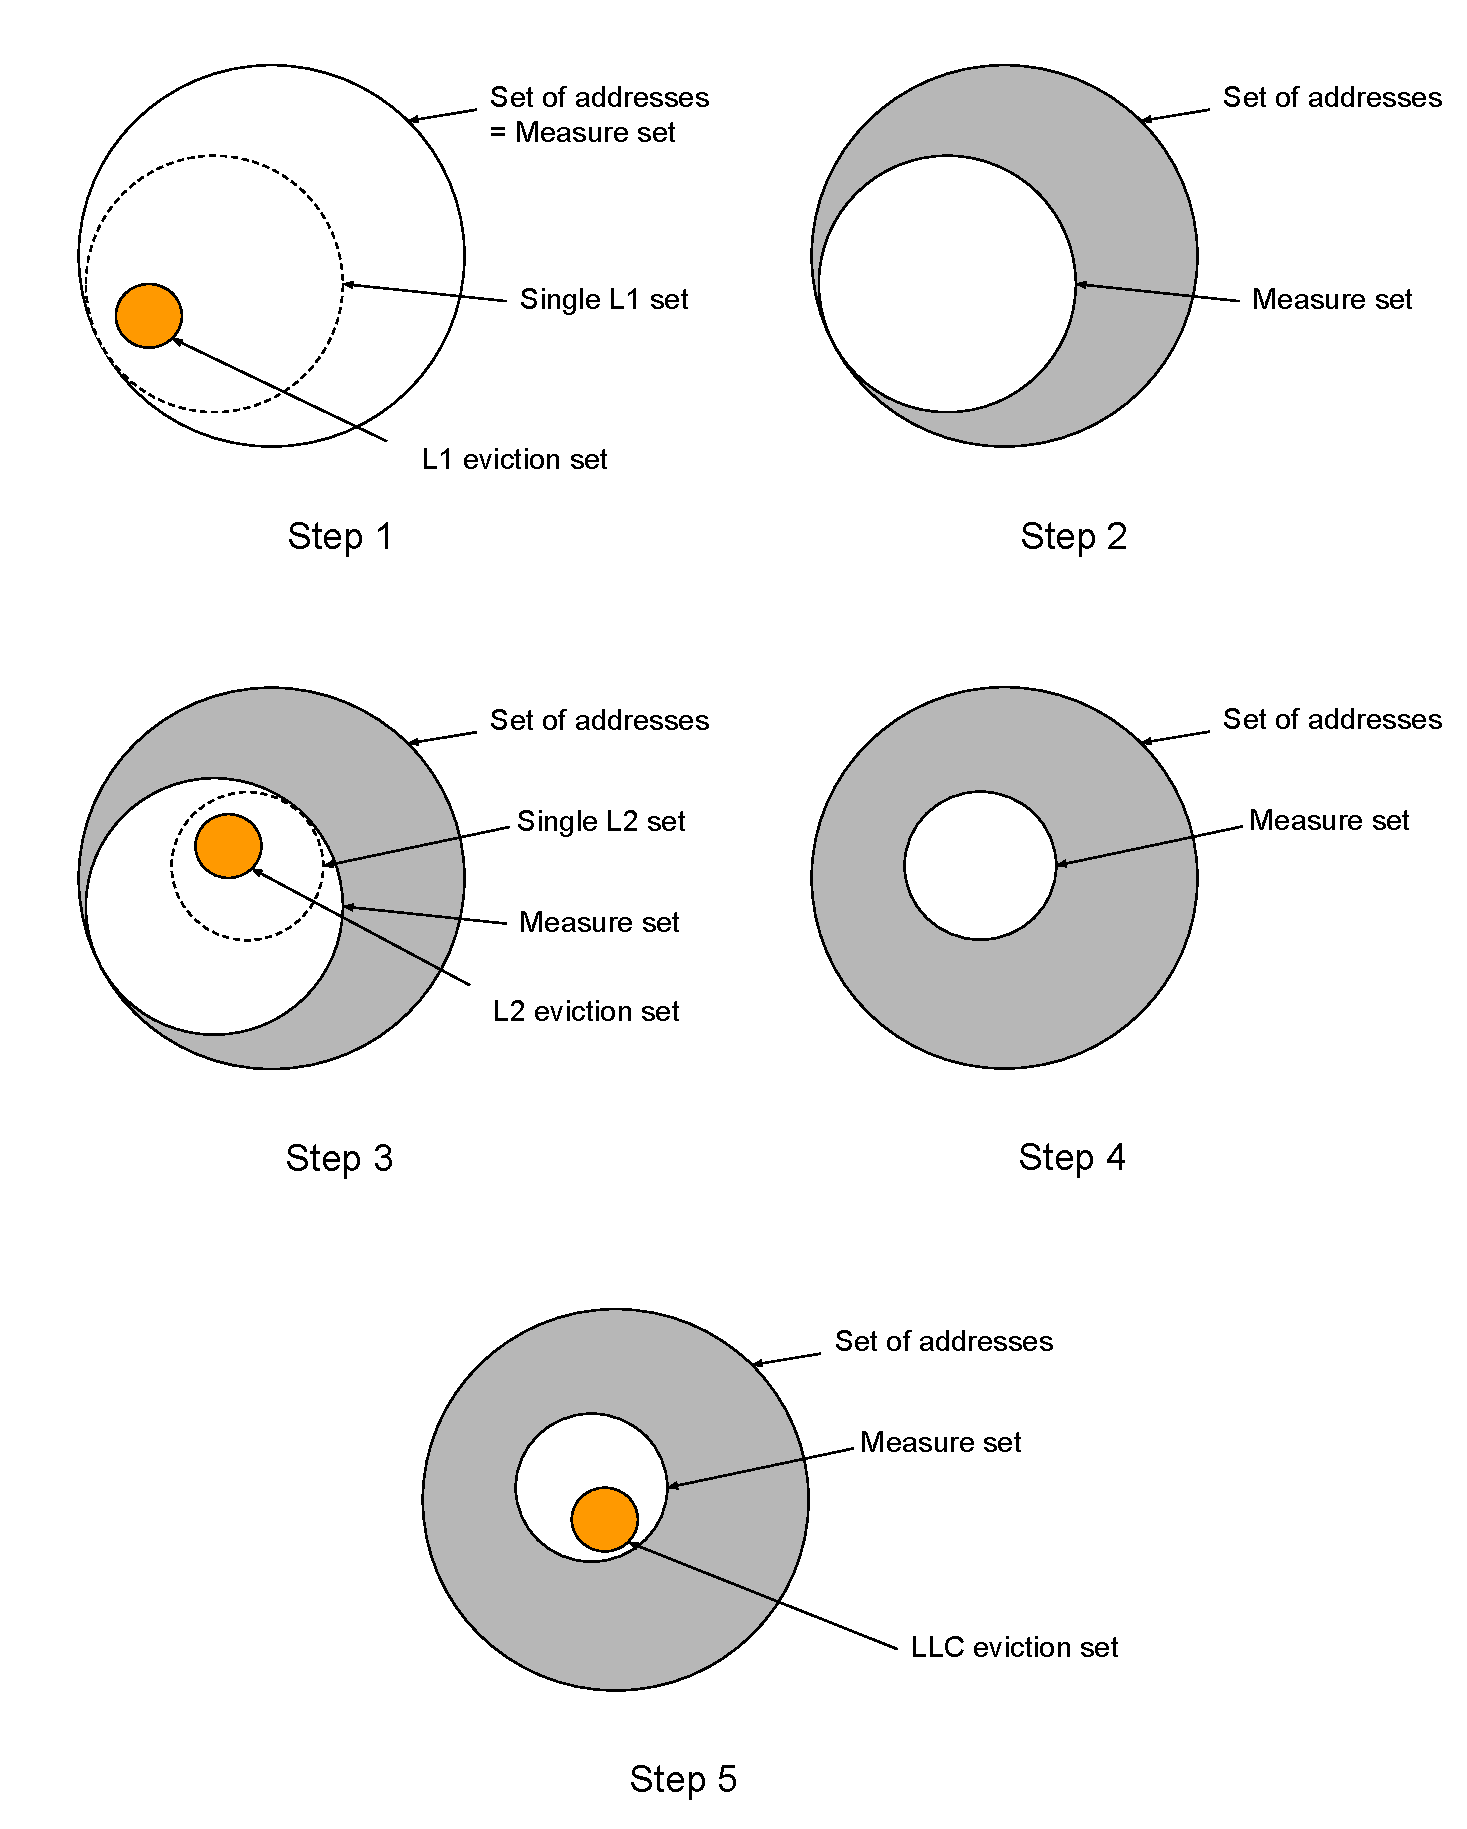
\includegraphics[width=15cm]{figures/illustrations/LLC_eviction_iterative.pdf}}
    \caption{Finding an LLC eviction set, without memory assumptions}
    \label{fig:llc_eviction_iterative}
\end{figure}

Thus, if we repeat the procedure using only this subset of addresses, we expect to quickly measure an L2 miss and find an L2 eviction set. Again, this gives us an oracle to distinguish addresses that map to this L2 set. The exact same steps can then be repeated to measure the associativity of every subsequent caches, including the LLC. The fact that the last shared cache might be physically separated into multiple slices do not invalidate the procedure. It simply means that we expect to explore more addresses before detecting an L3 miss. 

\autoref{fig:llc_eviction_iterative} illustrate the procedure to find an LLC eviction set, assuming the corresponding machine has three caches. The procedure begins at Step 1, with a fixed set of addresses. The algorithm will first detect an L1 eviction set, using the technique described in \autoref{sec:llc_eviction_simple}. Using this eviction set allows the algorithm to detect whether an address maps to the same L1 set as the eviction set. In Step 2, the algorithm can thus filter out the addresses that map to other L1 sets, and only consider the remaining addresses. In Step 3, the algorithm again finds an eviction set using the new measure set. This eviction set corresponds to an L2 eviction set. Again, this eviction set can be used to know which addresses map to the same L2 set as the L2 eviction set. In Step 4, only the addresses mapping to the same L2 set are considered, the others are discarded. Finally, in Step 5, the algorithm find an eviction set a third time, which will finally correspond to an LLC eviction set.

\subsection{Step Detection and Validation}

To measure a cache associativity, we first need to detect a miss corresponding to this cache. To do so, we will need to detect a step in the time function that is caused by a miss corresponding to the current cache. We observe the ratio of every two consecutive measures, and compare it to a certain threshold. This threshold should be small enough to detect every step, but not too small as to avoid detecting too many false positives. The problem is there is no such thing as a single perfect threshold. The more addresses we have in our measure set, the smaller we expect the step to be. Indeed, assume we have $n$ addresses in our set. When the corresponding blocks do not fit in the cache anymore, it is impossible to have $n$ consecutive cache hits. Thus, we expect to observe a miss ratio of at least $\frac{1}{n}$. It follows that with a bigger set, the miss ratio will diminish, and the threshold we need to use will also diminish. For this reason, we will detect steps using a dynamic threshold which is proportional to $\frac{1}{n}$, where $n$ is the number of addresses of the current measure. This way, we expect to correctly detect every step caused by a new eviction set while avoiding a maximum of false positives.

In practice, detecting an sudden increase in the time function is necessary, but still not sufficient. It is still possible to observe a sudden increase that does not indicate a new eviction set. In fact, every lower level cache is going to induce a step in the time function. The TLB will also induce steps in the time function.

For example, when trying to get an eviction set for the L2 cache, we only use addresses that map to the same L1 set. This reduces some irregular behaviour caused by the L1, but that does not mean it will not influence the measures. Indeed, when we access a number of addresses which is greater than the associativity of the L1, the time measured will suddenly increase because of the L1 misses, but this does not correspond to a new eviction set.

To differentiate a step caused by a new eviction set and a step caused by some lower cache or TLB, we can use the fact that the steps we are trying to recognise have a particular behaviour under certain circumstances. If we see an increase in the measures because a lower cache cannot hold all the blocks we are accessing, then no matter what the addresses in our set are, we will still observe misses. The reason is that we only use addresses that map to the same cache set, for any previous cache. This means that using a number of those addresses greater than the associativity of a previous cache will always result in misses, no matter which ones we choose. However, if the step is caused by a new eviction set (i.e., an eviction set corresponding to the current cache), then only a subset of addresses cause the cache set to overflow. Indeed, some addresses will map to the same cache set and cause it to overflow, but others might map to other sets such that no new set overflows This means that it is possible to remove the last address the algorithm added, and replace it by another one so that no more misses occur. If such an address can be found, then we know the step is indeed caused by a new eviction set. This gives us a way to eliminate some false positives when trying to detect steps causes by a new eviction set.

Another way to add robustness in order to avoid detecting false positives is to look at the newly found eviction set. When accessing only the eviction set and another address that maps to the same cache set, there will be cache misses. Since the address set is rather small, we expect to see a significant difference in the time necessary to access it compared to accesses that would result in only hits. One can indeed check that this difference is significant, and disregard the eviction set otherwise.

%%%%%%%%%%%%%%%%%%%%%%%%
\chapter{Implementation}
%%%%%%%%%%%%%%%%%%%%%%%%

%The implementation covers some of the implementation details of your project.
%This is not intended to be a low level description of every line of code that
%you wrote but covers the implementation aspects of the projects.

%This section is usually 3-5 pages.

To implement these algorithms in JavaScript (in order to be executed in a web browser), we first need to use a virtual region, or a set of addresses. To represent both, we will simply allocate an array that is roughly 1GB big. The array will then contain values that are contiguous in virtual memory, that we can use in the algorithms. To make sure the (unknown) physical placement of these addresses stay the same, we will use the same array for the whole experiment, instead of reallocating a new one every time. This way, we ensure that the physical addresses do not change through the whole algorithm.

\section{Precise measurement system}

In order to implement the precise timer system, we will use the built-in \texttt{performance.now()} clock system. By itself, this clock has a resolution that is too coarse to distinguish a cache miss from a cache hit. For example, Firefox 60 and its more recent versions use a resolution of 1 millisecond, but we would need a nanosecond precision in our experiments to distinguish a single hit from a single miss. Furthermore, jitter was added to this clock in most modern browsers, to help mitigate software vulnerabilities~\cite{aleph_spectre}. 

For this reason, we can implement an algorithm that is capable of measuring the time necessary to access multiple addresses consecutively by amplifying misses, while preventing some browser optimizations. It can be tuned to increase precision when necessary.

Algorithm~\ref{measure_algo} works by using a temporary \texttt{accessor} array, which we will use to generate the order in which the addresses will be loaded. Memory at each virtual address will then contain the address of the next block we will load, such that using the result of a load as the next address will result in a loop containing all of the input addresses. Note that in practice, multiple measures have to be taken, and the final measure is their average, to further increase precision. 

As an additional way to increase precision, the algorithm will first prepare the cache states by doing a full loop of accesses before measuring. The reason here is that we do not want to pollute our measures with additional cache misses. This way, we avoid measuring any unnecessary compulsory miss, and we will only have conflict misses or capacity misses.

\definecolor{CommentGray}{gray}{0.6}
\begin{algorithm}
\caption{Measuring Accesses Time}\label{measure_algo}
\hspace*{\algorithmicindent} \textbf{Input:} \texttt{addresses}\\
\hspace*{\algorithmicindent} \textbf{Output:} measured time
\begin{algorithmic}[1]
\Procedure{MeasureAccesses}{}
\State \textcolor{CommentGray}{// first phase: preparation}
\State \texttt{accessor $\gets$ [0, 1, ..., addresses.length-1]}
\State \texttt{accessor.shuffle()}
\For{\texttt{i $\gets$ 0; i<addresses.length-1; i $\gets$ i+1}}
\State \texttt{store(addresses[accessor[i]], addresses[accessor[i+1]])}
\EndFor
\State \texttt{store(addresses[accessor[addresses.length-1]], accessor[0])}
\State \texttt{idx $\gets$ load(addresses[0])} 
\State \texttt{junk $\gets$ 0}
\For{\texttt{i $\gets$ 0; i<addresses.length; i $\gets$ i+1}}
\State \texttt{idx $\gets$ load(idx)}
\State \texttt{junk $\gets$ junk + idx}
\EndFor
\State
\State \textcolor{CommentGray}{// second phase: measure}
\State \texttt{begin $\gets$ performance.now()}
\For{\texttt{i $\gets$ 0; i<nIter; i $\gets$ i+1}}
\State \texttt{idx $\gets$ load(idx)}
\State \texttt{junk $\gets$ junk + idx}
\EndFor
\State \texttt{end $\gets$ performance.now()}
\State \texttt{t $\gets$ end - begin}
\State \Return \texttt{(t, junk)}
\EndProcedure
\end{algorithmic}
\end{algorithm}

Algorithm~\ref{measure_algo} implements a pointer chasing method, to prevent optimizations. This means that every memory location it loads contains the address of the next block it will load, thus introducing dependencies between the loads, and forcing them to be serialized. The pointers form a random cycle which accesses every address in our set exactly once, to avoid any form of hardware prefetching. \autoref{fig:pointer_chasing} illustrates this method.

\begin{figure}
    \centering
    \fbox{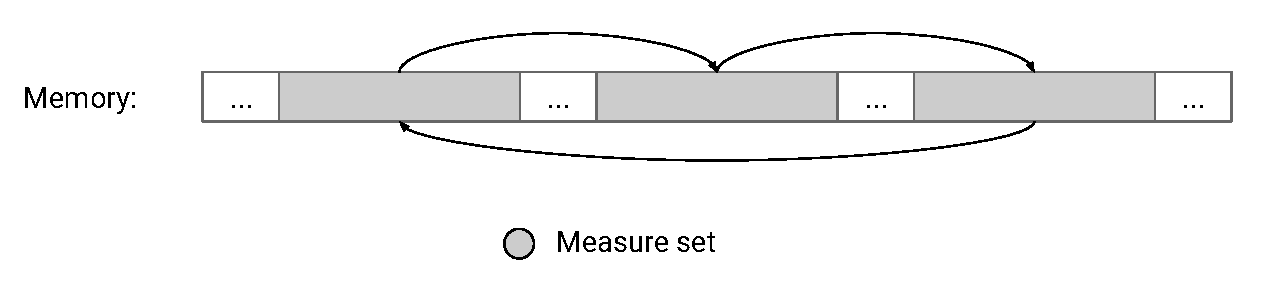
\includegraphics[width=15cm]{figures/illustrations/pointer_chasing.pdf}}
    \caption{Pointer chasing}
    \label{fig:pointer_chasing}
\end{figure}

It also keeps track of a \texttt{junk} variable which carries results from every memory load operation. This variable will then be returned or printed, so that memory accesses cannot be optimized away.

\section{Measure Cache Size}

Algorithm~\ref{size_algo} summarizes the procedure necessary to measure the cache size, given minimum and maximum region sizes to explore. The minimum and maximum sizes should cover all reasonably sized caches. The algorithm uses a virtual region of certain size (represented by an array) and progressively takes measures while increasing the size of the array. A simple optimization is possible here, since it is not necessary to access all addresses in a region. It is sufficient to access addresses separated by 64B. The reason is that a cache line is 64B long. All we need it to fetch every cache line, and since cache lines are 64B long, it is sufficient to load a single address every 64B in order to load every block in the virtual region.

\begin{algorithm}
\caption{Measuring Cache Sizes}\label{size_algo}
\hspace*{\algorithmicindent} \textbf{Input:} \texttt{min\_size, max\_size}\\
\hspace*{\algorithmicindent} \textbf{Output:} cache sizes
\begin{algorithmic}[1]
\Procedure{GetCacheSizes}{}
\State \texttt{T $\gets$ []}
\State \texttt{size $\gets$ min\_size}
\While{\texttt{size < max\_size}}
\State \texttt{S $\gets$ alloc\_region(size)}
\State \texttt{t $\gets$ \Call{MeasureAccesses}{S}}
\State \texttt{T.add(t)}
\State \texttt{size $\gets$ size + 1}
\EndWhile
\State \texttt{cache\_sizes $\gets$ get\_slope\_increase(T)}
\State \Return \texttt{cache\_sizes}
\EndProcedure
\end{algorithmic}
\end{algorithm}

Where procedure \texttt{get\_slope\_increase} is a function that takes an array of measures, and returns horizontal values where an increase in slope is detected, which will correspond to possible cache sizes.

\section{Measure Cache Associativity}

\subsection{With physical contiguous memory}

If we assume physical contiguity of virtual memory, algorithm~\ref{eviction_algo} describes a way to detect an eviction set, by using a set of addresses that all map to the same cache set, and by progressively increasing the number of addresses until we detect a cache miss. If the input \texttt{valid\_addresses} corresponds to a set of virtual addresses separated by a multiple of the size of a way of the cache, then the size of the resulting eviction set will be equal to the associativity of the cache, by construction. Note that it works even if the cache we are measuring is physically spread across multiple slices.

\begin{algorithm}
\caption{Finding An Eviction Set}\label{eviction_algo}
\hspace*{\algorithmicindent} \textbf{Input:} \texttt{valid\_addresses}\\
\hspace*{\algorithmicindent} \textbf{Output:} an eviction set
\begin{algorithmic}[1]
\Procedure{GetEvictionSet}{}
\State \textcolor{CommentGray}{// first phase: step detection}
\State \texttt{S $\gets$ \{\}} 
\State \texttt{A $\gets$ \{\}} 
\State \texttt{T $\gets$ []}
\While{no step detected in \texttt{T}}
\State \texttt{A = valid\_addresses.pop()}
\State \texttt{S.add(A)}
\State \texttt{T.add(\Call{MeasureAccesses}{S})}
\EndWhile
\State
\State \textcolor{CommentGray}{// second phase: eviction set isolation}
\State \texttt{E $\gets$ \{\}} 
\ForAll{\texttt{a $\in$ S}}
\State \texttt{t $\gets$ \Call{MeasureAccesses}{S $\setminus$ a}}
\If{\texttt{t} is "fast"}
\State \texttt{E.add(a)}
\EndIf
\EndFor
\State \texttt{E.pop()}
\State \Return \texttt{E}
\EndProcedure
\end{algorithmic}
\end{algorithm}

In practice, it is still possible that the algorithm incorrectly detects a step here, because of the noise. It is then necessary to add more robustness, to further increase the chances that the algorithm will succeed. After having found an eviction set, algorithm~\ref{eviction_algo} will try to isolate it. We can instead modify the algorithm so that it tries multiple times to isolate it, and if the results are not consistent it is likely that there is no eviction set yet, and it will thus go back and try to add addresses until it detects another valid step.

To tell which measures are faster and constitute the eviction set, it is often sufficient to use a k-means clustering algorithm with two clusters, since the two clusters are usually fairly distinct. The lower cluster will indicate the eviction set. For this reason, we choose to first take the measure for every address, and then only separate them in two clusters.

\subsection{Without physical contiguous memory}

Algorithm~\ref{enumerate_algo} summarizes the procedure to measure the associativity of the different caches while being executed by a web browser.
It proceeds as described above, by progressively finding eviction sets corresponding to lower caches, and using them to filter the addresses until finding the LLC eviction set.

As described earlier, the bigger the measure set is, the harder it is to detect a step in the time function. Furthermore, measure gets much noisier with the LLC, as it is shared. For this reason, the number of times a measure is taken will further increase by a factor proportional to the size of the measure set, to further reduce noise when necessary.

\begin{algorithm}
\caption{Enumerating Eviction Sets}\label{enumerate_algo}
\hspace*{\algorithmicindent} \textbf{Input:} \texttt{valid\_addresses}\\
\hspace*{\algorithmicindent} \textbf{Output:} all eviction sets
\begin{algorithmic}[1]
\Procedure{EnumerateEvictionSets}{}
\State \texttt{eviction\_sets $\gets$ []}
\For{\texttt{i $\gets$ 0; i < 3; i $\gets$ i+1}}
\State \texttt{new\_eviction\_set $\gets$ \Call{GetEvictionSet}{valid\_addresses}}
\ForAll{\texttt{a $\in$ valid\_addresses}}
\State \texttt{t $\gets$ \Call{MeasureAccesses}{new\_eviction\_set $\cup$ a}}
\If{\texttt{t} is "fast"}
\State \texttt{valid\_addresses.remove(a)}
\EndIf
\EndFor
\State \texttt{eviction\_sets.add(new\_eviction\_set)}
\EndFor
\State \Return \texttt{eviction\_sets}
\EndProcedure
\end{algorithmic}
\end{algorithm}

When the eviction set has been found, the algorithm needs to filter out all addresses that do not map to the same cache set as the eviction set. To do so, it will take a measure using the eviction set and the candidate address, as discussed earlier. It still needs to tell whether there are cache misses, but unlike algorithm~\ref{eviction_algo}, we cannot first take the measures with every address and then find the measures that do not have cache misses using k-means. Here, the amount of addresses that we would need to check can be much bigger than in algorithm~\ref{eviction_algo}. For this reason, we wish to tell whether a measure induces cache misses prior to taking further measures. 

To do so, it is possible to take reference measures during algorithm~\ref{eviction_algo}, when the eviction set have been found. The objective is to compute in advance an approximation of the time we expect to measure with an address that belong to the same cache set as the eviction set, as well as with an address that do not. This way, after having taken a measure with the eviction set and a candidate address, we could easily compare to both reference measures, and by choosing which one is the closest to the current measure, we would know whether there were cache misses.

All we need to compute reference measures are two addresses: one that maps to the same cache set as the eviction set, and one that does not. Using algorithm~\ref{eviction_algo}, we know that the very last address added to the set (the one which causes misses) is a positive example. It is then sufficient to take any address that was not recognised as part of the eviction set as a negative example. This way, we can easily compute reference measures.

Another main problem with this algorithm is that while searching for a new eviction set, the algorithm cannot tell whether there is still another eviction set that can be found, or we already have an eviction set for the LLC. This means that the algorithm could run for an unnecessarily long time without finding more results. In practice, this can be mostly be avoided by hard-coding a maximum number of eviction sets. Three seems to be a good choice, considering that most processors have three layers of caches. This means that the algorithm will not terminate on a processor with only two caches, and will not find all caches on a processor with more than three caches.

Algorithm~\ref{enumerate_algo} takes as input a set of addresses, but the choice of which addresses is important. In theory, we would only need addresses that map to the same L1 set, but in practice taking addresses separated by a greater stride (up to the size of a way of the LLC) still seems to increase physical alignment, as the algorithm converges faster. The problem is that the virtual region we have access to is limited, the size limit of an array that a browser is willing to allocate is around 1GB, meaning that we have a maximum number of addresses we can use. If we take a stride too big, the algorithm will converge faster, but we might not have enough addresses to find an eviction set for the LLC. On the other end, if we take a very small stride, we are almost sure that we will have enough addresses to detect the LLC eviction set, but the algorithm will take much longer to converge, and will have more chances to fail, given that the address sets will be bigger. As a temporary solution, taking a stride of 32KB seems to be a good enough compromise.

%%%%%%%%%%%%%%%%%%%%
\chapter{Evaluation}
%%%%%%%%%%%%%%%%%%%%

%In the evaluation you convince the reader that your design works as intended.
%Describe the evaluation setup, the designed experiments, and how the
%experiments showcase the individual points you want to prove.

%This section is usually 5-10 pages.

\section{Validation Using Huge Pages}

In order to validate the iterative approach of algorithm~\ref{enumerate_algo}, we first need to ensure that algorithm~\ref{eviction_algo} works as intended. Although we cannot check this directly in JavaScript since it requires some control over physical addresses (otherwise we would not need an iterative approach in the first place), it is possible to implement this algorithm in C using huge pages.

It would be possible to correctly run this algorithm using 2MB huge pages, but for the sake of completeness we will use 1GB huge pages. With a computer capable of using 1GB pages and configured to do so, it becomes possible to use a single 1GB page as a virtual region that will be mapped to a single 1GB contiguous page in physical memory. This way, we know that offsets of virtual memory within this region will be preserved in physical memory. We choose to implement this algorithm in C, because this language has support for huge pages, unlike JavaScript.

\begin{figure}
    \centering
    \fbox{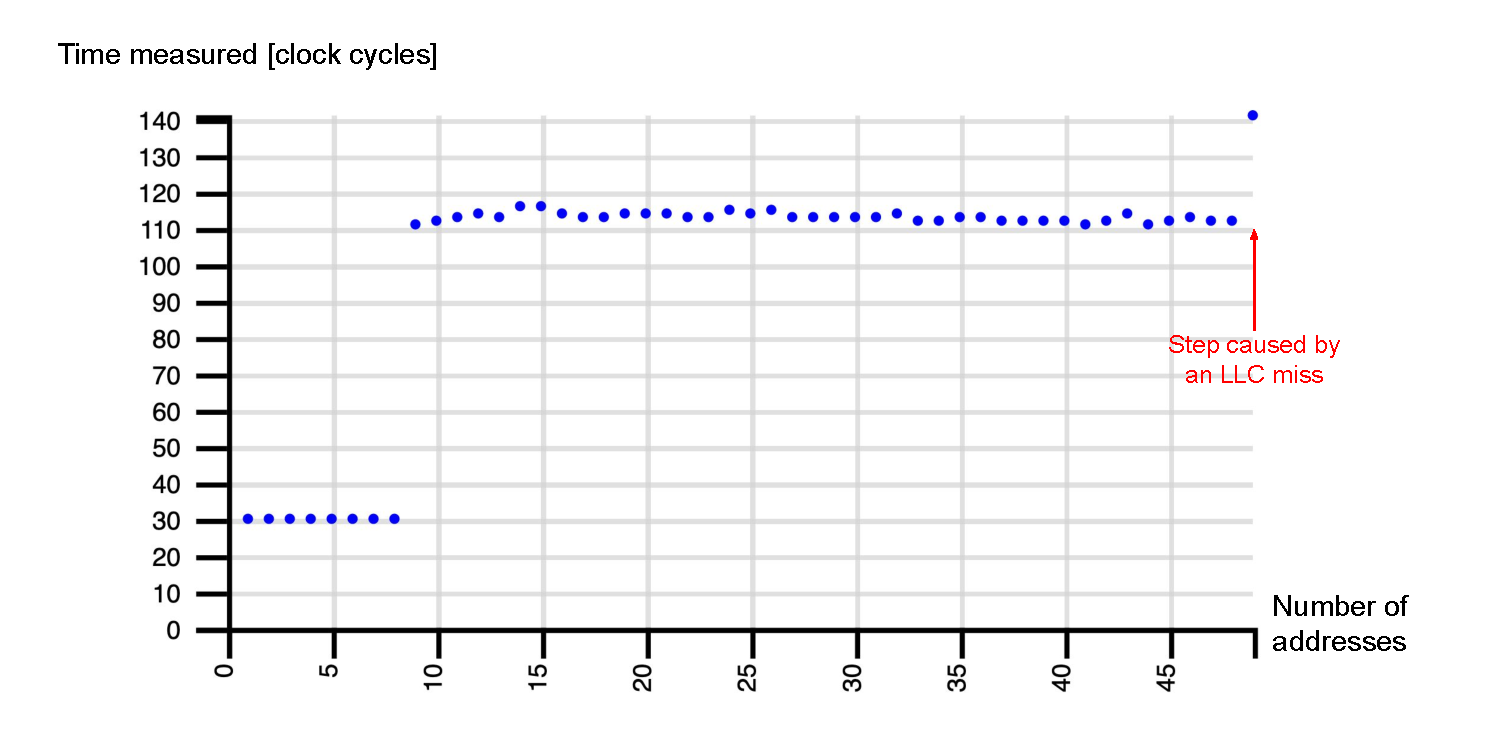
\includegraphics[width=15cm]{figures/results/4870HQ_c_eviction.pdf}}
    \caption{Detecting an LLC eviction set on an Intel Core i7-4870HQ, in c with huge pages. Notice the step at the last measure, which is caused by an LLC miss}
    \label{fig:4870_eviction_c}
\end{figure}

\begin{figure}
    \centering
    \fbox{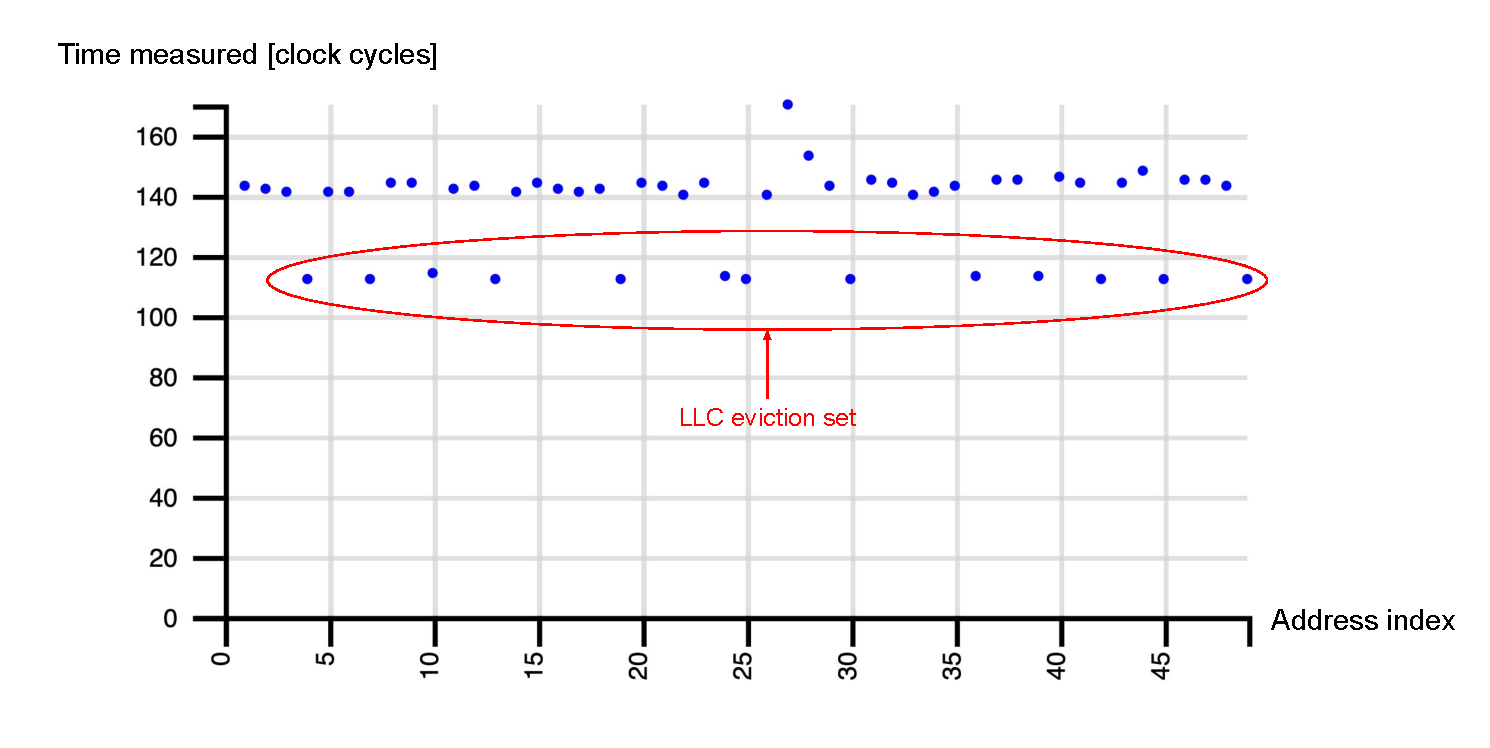
\includegraphics[width=15cm]{figures/results/4870HQ_c_associativity.pdf}}
    \caption{Isolating an LLC eviction set on an Intel Core i7-4870HQ, in c with huge pages. Notice the group of measure which are lower than the other measures. They correspond to an LLC eviction set}
    \label{fig:4870_associativity_c}
\end{figure}

\autoref{fig:4870_eviction_c} and \autoref{fig:4870_associativity_c} show the results of this algorithm implemented in C and executed on an Intel Core i7-4870HQ processor. On this machine, the size of a way of the LLC is 512KB, thus we only use addresses separated by 512KB to ensure that they all map to the same LLC set.

\autoref{fig:4870_eviction_c} shows the time measured with an increasingly big set of addresses. The last point in the graph corresponds to a step being correctly detected. Notice that a step at 9 addresses occurs but is not detected. It is caused by the fact that both the L1 and L2 cache are 8-associative, so L1 and L2 misses appear at 9 addresses. As described earlier, the algorithm could ignore this step due to the fact that no matter which 9 addresses are accessed, misses are always observed. Also note that since we are using huge pages, there are less virtual translations necessary here, and so the TLB does not overflow, and does not incur a step at 5 addresses, unlike in JavaScript.

\autoref{fig:4870_associativity_c} shows results of the second step of the algorithm, which tries to isolate the eviction set. It is fairly easy to distinguish the set of addresses which correspond to the eviction set here, because there is a clear separation into two clusters. The cluster constituted of the faster measures corresponds to the eviction set. It is made of 13 addresses, which matches the 12-associativity of the LLC in this case.

\section{Results}

\subsection{First experiment: cache size}

In the first experiment, we proceed as described in \autoref{sec:measure_cache_size}. The experiment will measure the time necessary to perform many memory accesses in an entire virtual region. In the following results, the virtual region size ranged from 1KB to 32MB, so any cache which size is in bounds should be detected. The x-axis constitutes the region size, and the y-axis the time measured. We expect to see sudden increase in slope near the size of the different caches.

When executed on an Intel Core i7-4870HQ using Firefox, the three caches are successfully detected. The cache sizes are 32KB, 256KB and 6MB. \autoref{fig:4870_size_l1} clearly shows the size of the L1 cache, which is 32KB big. 

\autoref{fig:4870_size_l2} shows the effects of the L2 cache. Notice how the slope increase is smoother than for the L1 cache. This is due to the fact that the measure set contains more addresses than previously, so the effect of a single miss influences less the final measure. Also note how the cache is 256KB big, but the slope increase happens around 220KB. This is mostly due to the fact that we have no control over physical translation of virtual addresses in JavaScript, and so our virtual region might not be contiguous in physical memory. A consequence is that addresses might not be evenly distributed among cache sets, and misses might occur with sets smaller than the cache size.

\autoref{fig:4870_size_l3} shows similar results with the LLC. The measures are much noisier due to the fact that this cache is shared, so cache pollution might occur. Similarly to the L2, the increase in slope occurs before 4MB, even though the L3 cache is 6MB big. It is still fairly clear that a cache of size close to 4MB is detected, although the exact size cannot be determined with those measures alone.

\begin{figure}
    \centering
    \fbox{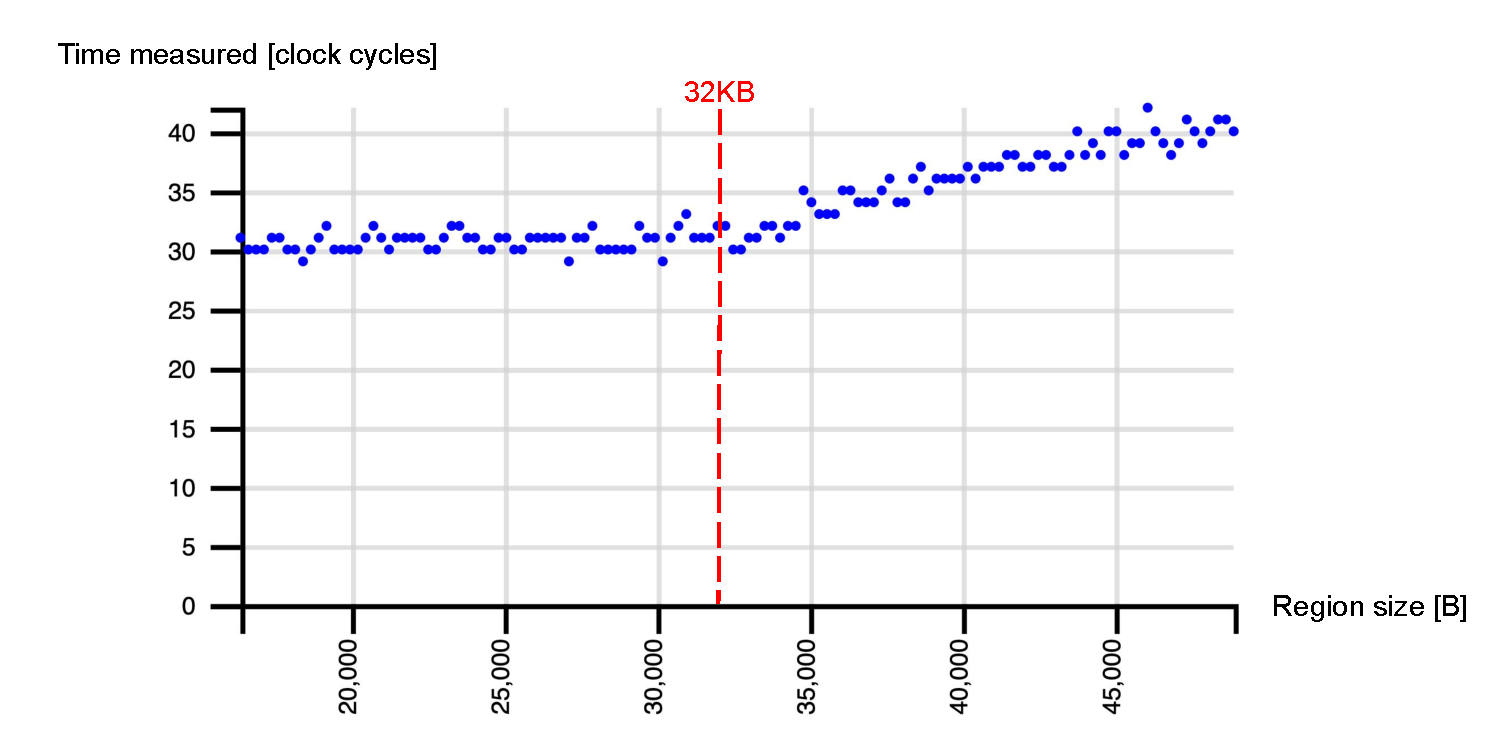
\includegraphics[width=15cm]{figures/results/4870_size_l1.pdf}}
    \caption{L1 size on an Intel Core i7-4870HQ in JavaScript. Notice the clear slope increase at 32KB, which corresponds to the L1 size}
    \label{fig:4870_size_l1}
\end{figure}
\begin{figure}
    \centering
    \fbox{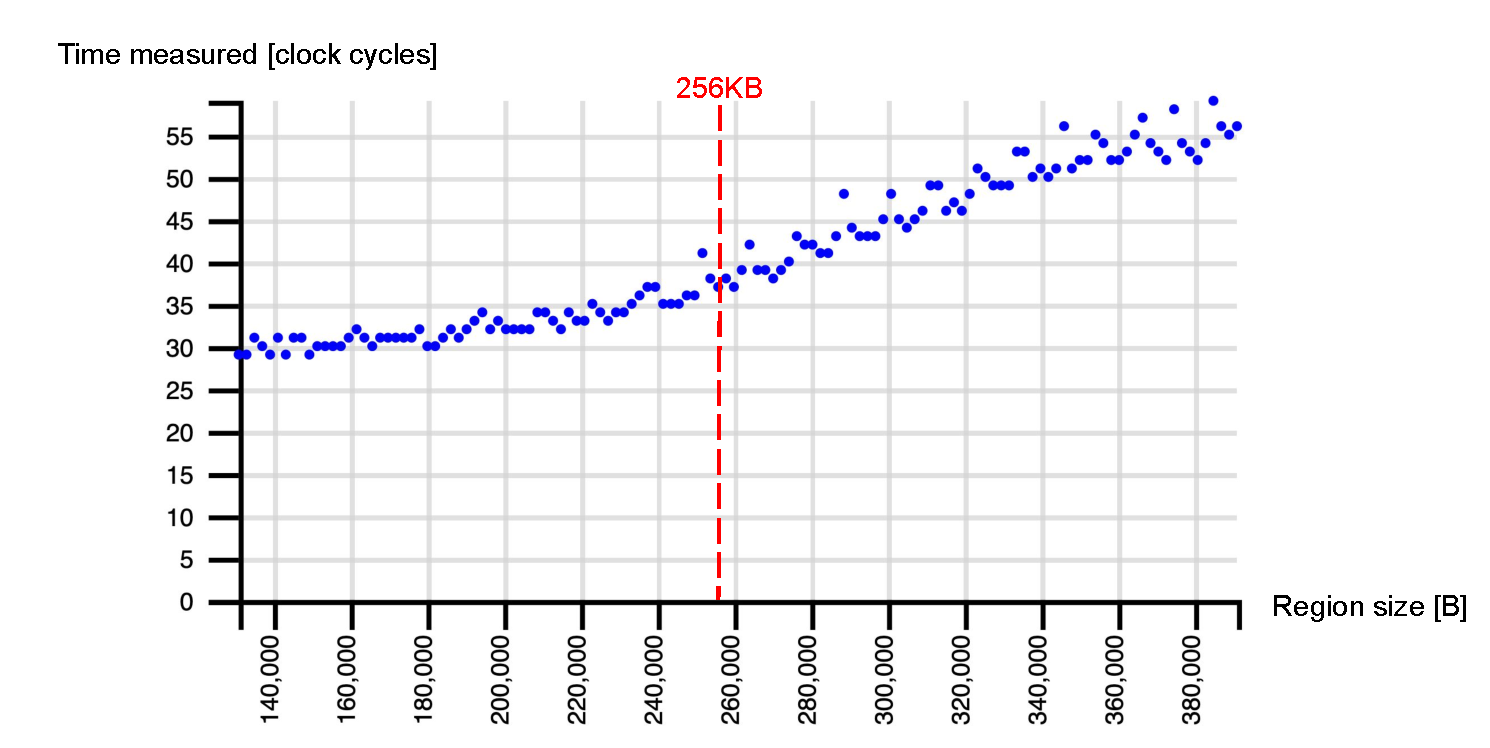
\includegraphics[width=15cm]{figures/results/4870_size_l2.pdf}}
    \caption{L2 size on an Intel Core i7-4870HQ in JavaScript. Notice how the slope increases progressively between 180KB and 260KB, whereas the L2 size is 256KB}
    \label{fig:4870_size_l2}
\end{figure}
\begin{figure}
    \centering
    \fbox{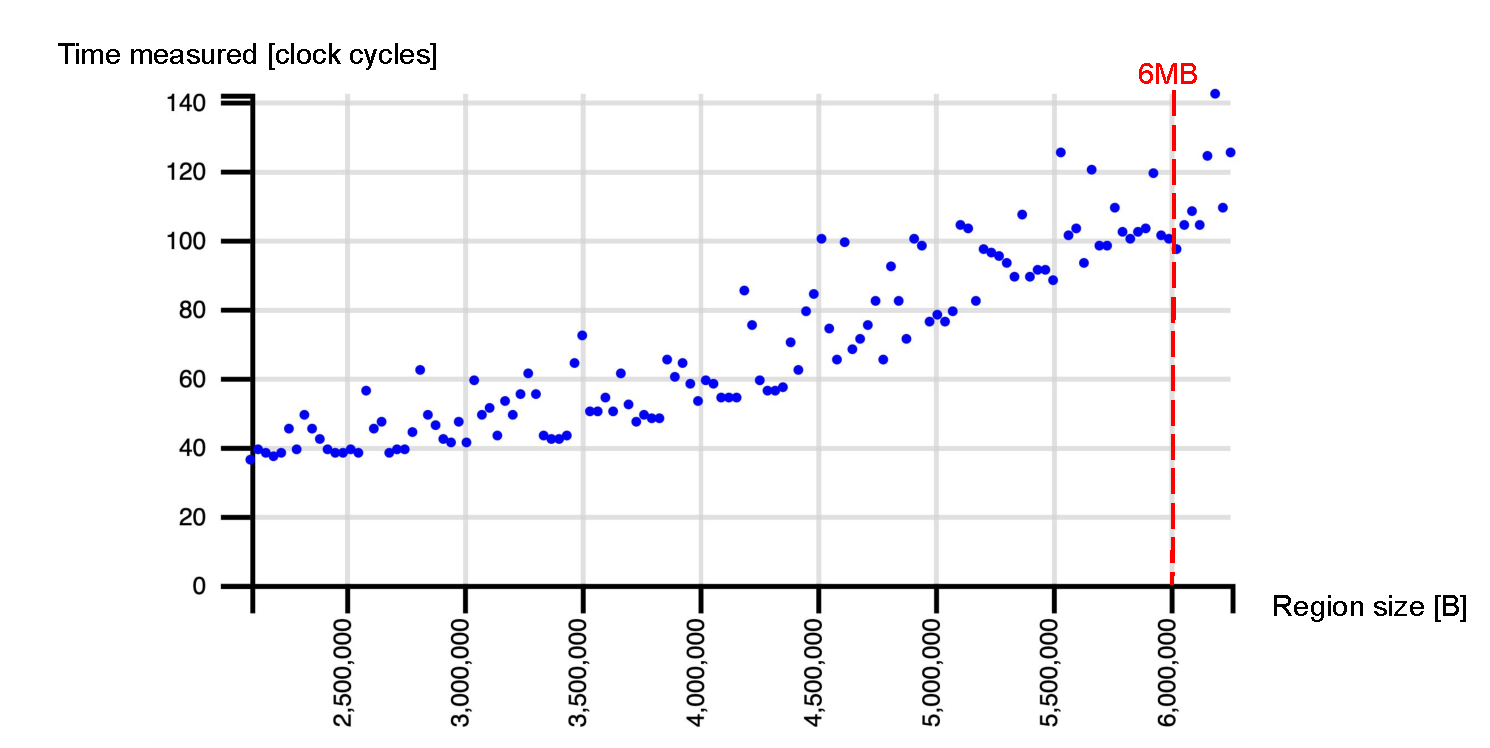
\includegraphics[width=15cm]{figures/results/4870_size_l3.pdf}}
    \caption{L3 size on an Intel Core i7-4870HQ in JavaScript. Notice how the slope increases progressively between 3MB and 5MB, whereas the LLC size is 6MB}
    \label{fig:4870_size_l3}
\end{figure}

\begin{table}
\centering
\begin{tabular}{ |p{3cm}||p{3cm}|p{3cm}|p{3cm}|  }
 \hline
 Processor model & Real L1 size / Measured L1 size [KB] & Real L2 size / Measured L2 size [KB] & Real L3 size / Measured L3 size [MB]\\
 \hline
 Intel Core i7-4870HQ & 32 / 32 &256 / 256&6 / 4\\
 \hline
 Intel Core i7-3610QM & 32 / 32  &256 / 256 &6 / 4 \\
 \hline
 Intel Core i9-9900K & 32 / 32 & 256 / 256& 16 / 8 \\
 \hline
\end{tabular}
\caption{Results of the first experiment, using Firefox 73}
\label{tab:cache_size}
\end{table}

\autoref{tab:cache_size} Summarizes results on multiple machines. All tests are ran using Firefox 73. All machines have three caches, so the L3 cache is also the LLC cache. The measured L1 / L2 / L3 cache represent the approximate point in the graph where the slope increases, rounded to the nearest power of two, by lack of precision. The algorithm consistently detects caches, but is mostly not capable of giving precise cache sizes when it comes to shared LLC.

\subsection{Second experiment: cache associativity}

For the second experiment, we will measure cache associativity using the algorithm described in \autoref{sec:measure_associativity}. As described, the algorithm will first try to overflow some L1 set, then isolate the corresponding L1 eviction set to get the L1 associativity. Iteratively, it will then repeat the process for L2 and L3 caches.

When executed on an Intel Core i7-8700 using Firefox, the algorithm could correctly measure the associativity of last level cache, despite the high amount of noise.

\begin{figure}
    \centering
    \fbox{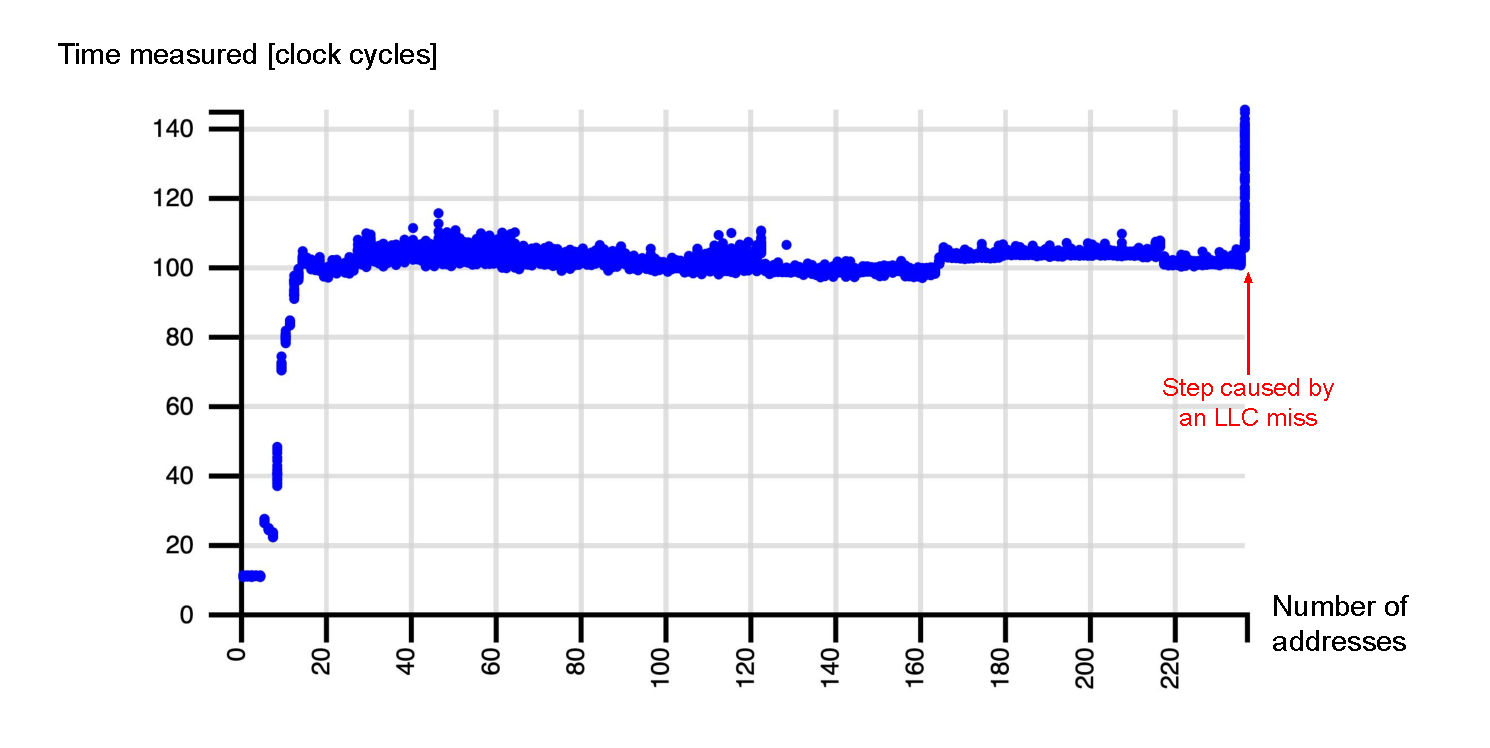
\includegraphics[width=15cm]{figures/results/8700_eviction_L3.pdf}}
    \caption{Detecting an LLC eviction set on an Intel Core i7-8700 in JavaScript. Notice the step at the last measure, which is caused by an LLC miss}
    \label{fig:8700_eviction_L3}
\end{figure}

\autoref{fig:8700_eviction_L3} shows the results of the first phase of algorithm~\autoref{eviction_algo} on this machine, while measure the associativity of the L3 cache. The first phase uses an increasing number of addresses, until detecting a step corresponding to a miss in the current cache. X-axis depicts the number of addresses used. Y-axis shows the time necessary to access all of these addresses a fixed number of times. Notice the steps around 4 and 8 addresses caused respectively by the associativity of the TLB and the previous caches. Also note the steps that do not correspond to L3 misses, but rather noise, as the measures settle down again afterwards.

\begin{figure}
    \centering
    \fbox{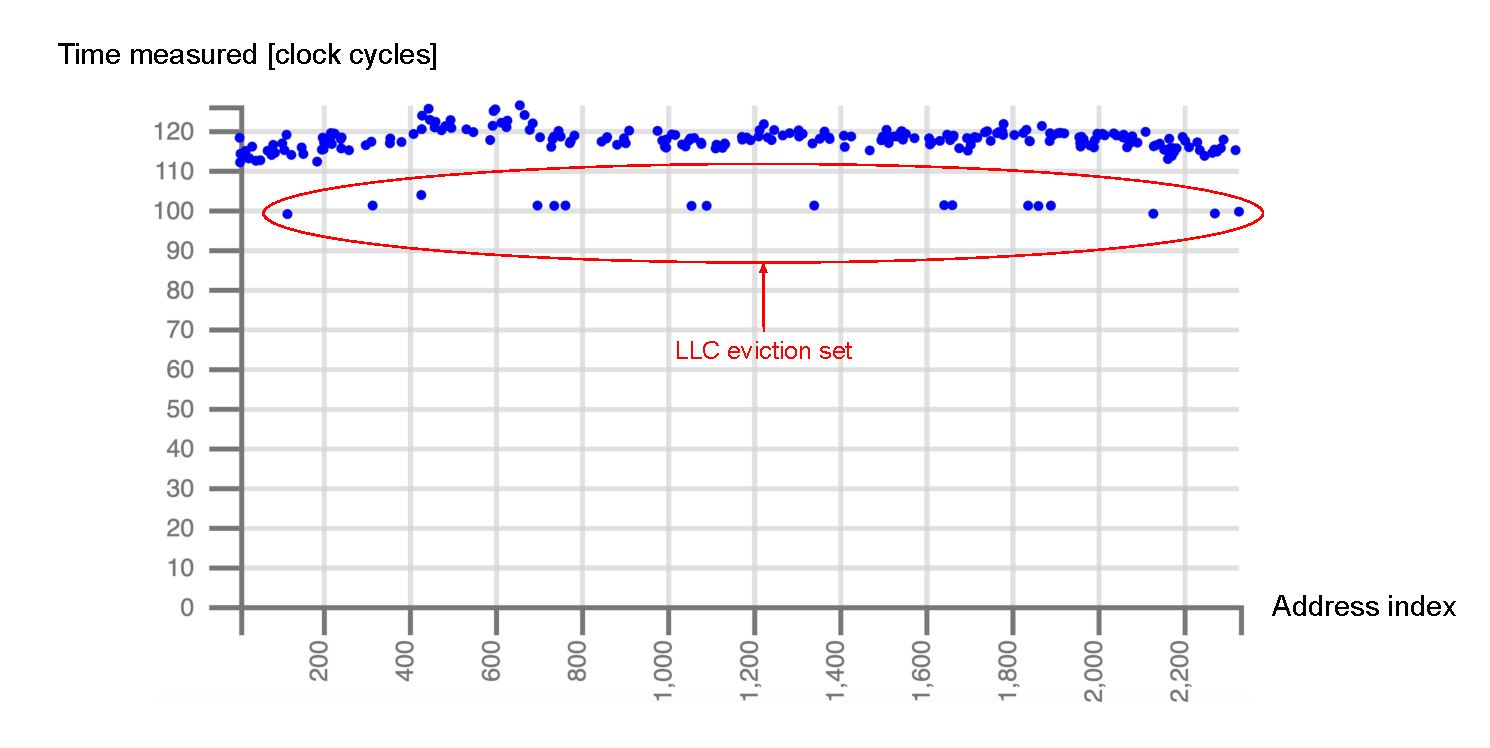
\includegraphics[width=15cm]{figures/results/8700_associativity_L3.pdf}}
    \caption{Isolating an L3 eviction set on an Intel Core i7-8700 in JavaScript. Notice the group of measure which are lower than the other measures. They correspond to an LLC eviction set}
    \label{fig:8700_associativity_L3}
\end{figure}

\autoref{fig:8700_associativity_L3} shows the second phase of the algorithm, while isolating the eviction set to get the associativity. X-axis depicts the index of the candidate address, as described in \autoref{sec:cache_associativity_no_contig}. Despite the high amount of noise, the eviction set still appears quite clearly, and the 17 measures that are below the others indeed correspond to the fact that this cache is 16-associative.

\begin{table}
\centering
\begin{tabular}{ |p{3cm}||p{3cm}|p{3cm}|p{3cm}|  }
 \hline
 Processor model & Real L1 associativity / Measured L1 associativity & Real L2 associativity / Measured L2 associativity & Real L3 associativity / Measured L3 associativity \\
 \hline
 Intel Core i7-4870HQ & 8 / 8 &8 / 8&12 / 12\\
 \hline
 Intel Core i7-8700 & 8 / 9 & 4 / - & 16 / 16\\
 \hline
 Intel Core i7-3610QM & 8 / 8 &8 / 8&12 / 12\\
 \hline
 Intel Core i9-9900K & 8 / - &8 / -&12 / -\\
 \hline
 Intel Core i7-10510U & 8 / - &8 / -&12 / -\\
 \hline
\end{tabular}
\caption{Results of the second experiment, using Firefox 73}
\label{tab:cache_associativity}
\end{table}

\autoref{tab:cache_associativity} summarizes results obtained with this algorithm on different machines. Some observations can be done here. For example, it has been noticed that recent Intel processors (which include Intel Core i9-9900K and Intel Core i7-10510U) consistently fail to even detect the first eviction set. Some necessary assumption seems to be violated on these architectures, but it is unclear which one. Since the algorithm cannot detect the first eviction set, it cannot find any following eviction set either.

When it comes to the Intel Core i7-8700, the algorithm ran into a large amount of noise during detection of the L1 associativity. A consequence is that some measures were influenced by noise and mistaken as part of the eviction set, so the eviction set contains one address that does not belong to the eviction set, and the measure of the associativity is 9 instead of 8. Nonetheless, subsequent measures are not affected since this set is a super set of the eviction set. The fact that the L2 associativity is smaller than the L1 associativity also causes problems during the algorithm, and the second eviction set that was found corresponded to the L3 cache, effectively skipping the L2 cache. The associativity of the L3 cache is still correctly measured despite this fact.

Notice that every size or associativity that is correctly measured could allow to fingerprint a computer. It could for example be used with a given set of computers. If the architectures have different enough cache characteristics, the algorithms could be executed to recognize a single computer, by telling which computer corresponds the most to the measured values.

\section{Limitations}

There are still known cases where an algorithm will not produce correct results, depending on the machine or the browser.

When the algorithms are executed on Safari (both algorithms~\ref{size_algo} and \ref{enumerate_algo}), the measures will not show anything, as all the measures look constant. Safari seems remove the memory accesses, even though we tried to prevent such optimizations.

On the most recent Intel processors (starting from 2019), algorithm \ref{enumerate_algo} will consistently fail. Examples of such processors are the Intel Core i9-9900K or the Intel Core i7-10510U. On such processors, it will consistently fail to even fail to detect the first eviction set. When trying to add addresses to detect misses, it will still detect sudden increase in the measures but then cannot find the corresponding eviction set for an unknown reason. Nonetheless, Algorithm~\ref{size_algo} can still measure cache size.

Another kind of architecture which causes problems are the processors which have a cache with an associativity that is smaller than the previous caches. For example, if the L1 is 8-associative, but the L2 is only 4-associative. If this is the case, algorithm~\ref{enumerate_algo} can effectively miss the caches whose associativity is smaller than the previous ones, although it will still get an eviction set for the following caches. Such an example can be found with the Intel Core i7-8700. The algorithm managed to find an eviction set corresponding to the L1 cache, but the next eviction set it found corresponds to the L3 cache, skipping the L2.

Even on processors where the algorithm works, many iteration are necessary to get precise enough measures, because of the noise (for example from the fact that a cache might be used by another process, or the possible jitter added to the clock we use). The consequences are that algorithm~\ref{enumerate_algo} takes a significant amount of time to execute (it can take an entire day to complete), and it is still possible to fail some crucial measures mutliple times, which ultimately invalidates further results.


%%%%%%%%%%%%%%%%%%%%%%
\chapter{Related Work}
%%%%%%%%%%%%%%%%%%%%%%

%The related work section covers closely related work. Here you can highlight
%the related work, how it solved the problem, and why it solved a different
%problem. Do not play down the importance of related work, all of these
%systems have been published and evaluated! Say what is different and how
%you overcome some of the weaknesses of related work by discussing the 
%trade-offs. Stay positive!

%This section is usually 3-5 pages.

%https://alephsecurity.com/2018/06/26/spectre-browser-query-cache/

The article "Overcoming (some) Spectre browser mitigations"~\cite{aleph_spectre} was published after the Spectre and Meltdown mitigations, and showed those attacks were still partly applicable. It works in JavaScript and exploits speculative execution of a function to recover a secret value, using precise time measures. Although its objective is not the same as ours, this article introduces most necessary information to build a precise measurement system in JavaScript. It describes a way to use \texttt{performance.now()} and perform many memory accesses to see whether cache misses occurred, and infer cache information.

Although the measurement system differs a bit from ours, the basis is the same, and this article shows how to try to counter some browser optimizations (mostly by preventing dead code elimination and ensuring memory accesses are serialized). The main difference is that this algorithm uses a setup which ensures that the memory accesses result in either only hits or only misses. However, we cannot achieve this in our setup, while looking for eviction set. In our case, the miss rate in both cases will mostly be either zero, or small (and thus harder to differentiate).

Nonetheless, it offers a complete way to take precise enough measures in JavaScript with very little adjustments. Its only prerequisite is the ability to amplify misses, which we will also offer. Those measures allow us to distinguish two different cases, whether cache misses occur or not. This is the main way to detect cache misses that we use in this entire report.

%https://pdfs.semanticscholar.org/fe1d/d24acbed62497264b59f4b70ed4cfb321a9d.pdf

The master thesis called "Measurement-based Inference of the Cache Hierarchy"~\cite{abel} infers cache characteristics by performing timing measures. It manages to measure cache size and associativity of private and shared caches, as well as the block size and cache replacement policy. While this work could successfully measure those characteristics, the main difference is that this work relied on the fact that it was capable of counting the number of cache misses, given a certain set of addresses and an initial cache state.

Nonetheless, some of the algorithms necessary to measure cache characteristics it describes can still be used in JavaScript. In particular, the algorithms to measure the cache size and the (non physically indexed) cache associativity can be almost directly used, provided we have a way to tell whether cache misses occurred. The first algorithm can almost be used as-is in JavaScript. The only difference is that we are not as precise as if we were counting cache misses. In our case, we cannot directly detect a "step" corresponding to a capacity miss, as they do. What we do instead is continue to take measures by increasing the size of the measure set, and finally observe the graph to detect a sudden increase in slope. The second algorithm gives us the basis to measure cache associativity, although it is not directly applicable without assumptions on the virtual address translation, as we cannot always control to which cache set an address will be mapped. For this reason, we used this algorithm as a basis and modified it to then isolate the eviction set, which we can then use in JavaScript to measure the L1 associativity.

It also describes the benefits of using pointer chasing while performing memory accesses, to increase their precision, which we also applied for similar reasons.

%https://arxiv.org/pdf/1810.01497.pdf

A paper called "Theory and Practice of Finding Eviction Sets"~\cite{eviction_sets} provides a complete explanation of cache eviction sets, and presents a few algorithms to directly measure them from software. Like most related work, it relies on the fact that is can reliably take measures precise enough to tell whether a single memory access resulted in a miss, or in a hit. Although we are not as precise as that, we can still apply some of their algorithms in JavaScript.

More specifically, it fully describes the eviction sets, and tells us why the previous simple algorithms to measure cache associativity will mostly not work with the LLC. Most importantly, is provides an algorithm capable of isolating an eviction set, which is what we need to measure associativity in JavaScript. Their algorithm provides a first intuition on to how to implement a JavaScript equivalent version, by taking every address in the candidate set individually and checking whether removing it from the set and taking a measure results in only cache hits. The different behaviours of the measures will be sufficient to indicate whether an address is in the eviction set.

%https://eprint.iacr.org/2015/690.pdf

The article "Systematic Reverse Engineering of Cache Slice Selection in Intel Processors"~\cite{slice_reverse_engineer} provides a more concrete use of detecting eviction sets, as they use it as a way to reverse-engineer the LLC hashing function that maps an address to a slice, although they also need a way to tell cache misses and hits apart and is not implemented in JavaScript. Even though we do not infer the hashing function here, they provide a full method that can almost directly be implemented in C and using huge pages, for validation purposes.

Their algorithm can also be slightly adapted to work in JavaScript. The main difference is that instead of individually testing whether removing an address from the candidate set and taking a measure results in a miss, we first take a measure for every address and then we compare them to each other to determine which one of them resulted in only cache hits, using for example a k-means algorithm. As discussed earlier, this method requires control over virtual to physical translation, so this algorithm can only be used to directly measure the first level cache associativity. We still needed to find an iterative approach to also measure other caches, up the the LLC, included.

%https://etd.ohiolink.edu/!etd.send_file?accession=osu1308256764&disposition=inline

A thesis called "Robust Method to Deduce Cache and TLB Characteristics"~\cite{tlb_characteristics} describes methods to measure many hardware characteristics from software, including cache size and associativity, but also cache line size, word size and TLB size and associativity. Although they measure more characteristics than we do, they rely on the fact than a certain part of virtual memory is contiguous in physical memory, using 1MB huge pages, so their algorithms are not applicable in JavaScript directly.

Nonetheless, they provide very clear results that show the effects of the TLB on the measures. Those results were particularly useful during development, as they provided precious information on some previously unexplained behaviours. More specifically, they explain why some steps were incorrectly detected while trying to measure cache associativity, or even why some eviction sets can be found but do not correspond to any cache eviction set. The reason is that the TLB behaves like a cache in those experiments. The TLB also suffers from capacity misses and conflict misses, and those can in fact be mistaken for cache misses.

The similarity of behaviour between cache and TLB can in fact help us detect a TLB eviction set in JavaScript using the same algorithm under certain circumstances, but it also means that we sometimes isolate a TLB eviction set when we are in fact looking for a cache eviction set. This means that further measure are invalidated, since we did not find a lower cache eviction set, as necessary to measure the following caches.

%%%%%%%%%%%%%%%%%%%%
\chapter{Conclusion}
%%%%%%%%%%%%%%%%%%%%

%In the conclusion you repeat the main result and finalize the discussion of
%your project. Mention the core results and why as well as how your system
%advances the status quo.

In conclusion, those algorithms can sometimes fully detect cache size and associativity for all caches, including the shared LLC. For example, it achieves such results on an Intel Core i7-4870HQ, where it correctly measures every cache associativity, and can approximately detect cache sizes.

The algorithms still heavily depends on the underlying architecture. Even though it will mostly measure cache associativity on some computers, it will still reliably fail on others, such as recent Intel processors \footnote{such as Intel Core i9-9900K and Intel Core i7-10510U}, where it will even fail to detect a first eviction set. Furthermore, there is still a considerable amount of noise, due to the fact that the clock we are using is jittered, and because the caches might be polluted by some other processes. In consequence, the algorithms (and especially algorithm~\ref{enumerate_algo}) are never guaranteed to succeed, even with a high number of measures. It is always possible to fail key measures such that no results are found.

Nonetheless, on some architectures, the algorithms are fully capable of measuring both cache size and associativity in JavaScript, in a web browser, despite the fact that the web browser executes the code in a sandbox that is supposed to be as isolated as possible from the machine it is executing on. Measuring cache characteristics in software has already been done in previous works, but this project showed that it is still technically possible to measure them from within a web browser, and that it might be possible to extend these algorithms in future works

\cleardoublepage
\phantomsection
\addcontentsline{toc}{chapter}{Bibliography}
\printbibliography

\end{document}